\chapter{Theoretical Part -- Storage}\label{ch:storage_theory}
\section{Storage Abstractions}
Storage systems have evolved from simple, basic designs that meet basic criteria to modern systems intended to satisfy the needs of the modern computing era. This and the following sections will focus on explaining the basics of storage solutions, their evolution, and the emergence of the need for distributed storage. This should help the reader better understand how storage systems have evolved and highlight the needs that led to the creation of the software-defined storage principle.

Traditional storage solutions can be categorized into three main types (block storage, file systems, and object storage), each of which provides different needs with its own abstraction layer.

\subsection{Block Storage}
Block storage represents a foundational abstraction layer in modern computing and server architectures. It provides an abstraction layer for various physical storage systems, such as hard drives, solid-state drives, and storage networks. This abstraction allows a separation between the physical implementation of the underlying storage solution and the logical understanding of the provided storage. Consequently, this offers an easy communication interface between storage architects who deal with low-level solutions and infrastructure, and application architects who use that storage for their needs.

Block storage devices transform the storage layer into fixed-size logical blocks. These blocks are usually referenced via linear addressing, allowing applications to access precise parts of the devices. This allows almost complete access to the logical storage provided by the low-level architecture. This type of access does not limit applications or users in any way. The user of the block device is usually expected to manage and organize the data in the underlying storage themselves.

Direct use of block storage is often preferred for IO performance-sensitive applications, since it allows direct access to storage, and the organization of data can be tuned in any form that suits the application's needs.

Databases such as Oracle, Aerospike, and others use direct access to block storage devices. This allows those systems to manage their data structures directly. This can lead to optimizing memory operations by correctly serializing data in storage and implementing logic directly on the device. \cite{oracle_storing_2025, aerospike_ssd_2024} 

Direct access to block storage often requires complex implementation and requires a deep understanding of low-level concepts. However, specifically designed storage for specific use cases can lead to optimized storage access.

Although specialized applications use it directly, block storage is more commonly used as a building block for higher-level storage layers and abstractions. One such abstraction is a file system, which maps blocks of memory to files, directories, and other structures.\cite{muzikar_zarizeni_2025}

\subsection{File Systems}
The most common and well-known storage abstraction built on top of block devices is a file system. This abstraction layer introduces a familiar hierarchical structure of files and directories (or folders). Data are encapsulated in files (as logical units of data) and subsequently organized within a nested directory structure. A specific file is addressed using a path that defines a unique route through this hierarchy. Even though most users intuitively understand this model, its underlying implementation is significantly more complex than other storage abstractions, such as object storage.

This abstraction is comfortable because it shields the user and the application from the physical complexities of data storage. Instead of interacting with raw block addresses, the system interacts with logical files. The implementation of a file system is responsible for managing all low-level complexities, such as the placement of physical data and block allocation. This file-level and directory-level structure also simplifies higher-level operations, such as backups and replication, since these can be performed directly on the logical constructs (folders and files). \cite{muzikar_systemy_2025}

Another nice feature of file systems is native support for metadata. In most common file system implementations (POSIX-based), each file and directory maintains a set of metadata, which typically includes ownership (user, group), access permissions, timestamps (access, modification, change), and block pointers. For a large file, this metadata is negligible; however, for small files like images, the metadata (e.g., the inode and directory entries) can consume a large amount of space and, more importantly, a separate I/O operation to access.\cite{beaver_finding_2010}

It may seem that abstracting storage into files and folders is a clever and intuitive way to structure data, but such a solution also has drawbacks regarding performance and scalability. The first major drawback is the latency introduced by hierarchical path-based addressing. To read a single file, the file system must walk the entire path from the root \cite{beaver_finding_2010}. In common implementations, the (so-called) walk process involves accessing multiple structures stored on disk to finally access the needed data. In the case of XFS, the system must traverse the hierarchy, like in the following example:
\begin{quote}
\texttt{/}\\
\texttt{/folder/}\\
\texttt{/folder/subfolder/}\\
\texttt{/folder/subfolder/data.file}
\end{quote}
Such a walk often generates significant metadata overhead and I/O operations that are (in most cases) not needed by applications operating on the storage system.\footnote{Modern systems heavily rely on cache; Walk overhead is present only in cold cache systems or non-systematically accessing a large amount of files. This thesis addresses the problem of large amounts of data, so the walk issue remains valid.} \cite{beaver_finding_2010}

Another significant drawback of file systems is that they are designed for isolated single-node environments. To guarantee consistency of its internal structures and prevent data corruption due to race conditions, the file system must rely heavily on locking. This mechanism often forces the serialization of many operations. This serialization occurs when writing to the same file, modifying the same directory, or concurrently modifying the metadata \cite{yuan_introduction_2020}. Although it is not necessarily a problem in non-shared storage solutions and personal systems, the latency caused by locking may be significant in shared file systems on the network, where locks must be performed over the network. This may lead to weak performance in distributed solutions. \cite{liu_evaluation_2018}

\subsection{Object Storage}
Object storage is a relatively simple abstraction for managing data at scale. Its fundamental unit is the object. An object is a self-contained entity that contains raw data, descriptive metadata, and a unique identifier. Objects are organized in a flat namespace (known as buckets or collections) as an unordered set. Each object in a collection has a unique identifier by which it can be addressed. Some implementations may simulate hierarchical structures by embedding slashes in object names; however, from a design perspective, the namespace remains logically flat and no hierarchy is applied. \cite{mesnier_storage_2003}

Data are stored as raw binary data (the object's content) on the underlying storage systems. The data for one object are atomic and treated as a single data chunk. That makes operations with objects simple, such as writing or reading the whole object -- updates of some part of the data are typically not allowed. \cite{mesnier_storage_2003}

Having a unique key that addresses raw data essentially forms storage systems that can be treated as simple key-value stores.

The core component that realizes this abstraction is the object store. The object store is a service that orchestrates storage and maps object names, their metadata, and their physical locations. It can be considered as a database engine that implements the described key-value storage. The object store is responsible for maintaining the mapping between object identifiers and their physical placement, orchestrating data and metadata operations between storage nodes, and enforcing consistency, durability, and access policies. \cite{mesnier_storage_2003}

Object storage is a simple abstraction that enables higher-level use cases for users and applications. At its core, it has just three simple rules.
\begin{itemize}
    \item \textbf{Atomicity of an object} \\
    Each object is atomic and treated as an indivisible unit of data. The only supported operations are write, read, and delete of the whole objects. The data inside the object can be any binary data of any size or length (blob).
    \item \textbf{Unique Identifier} \\
    Every object is associated with a unique identifier (key) within its namespace, which is used to address it. This key abstracts away the physical location of the data and enables simple key-value-style operations for clients.
    \item \textbf{Object store as an orchestration} \\
    The object store is a service that manages the global namespace, metadata, and placement of objects across storage nodes. It orchestrates data and metadata operations, enforces consistency, durability, and access policies, and abstracts key values on top of the underlying storage resources.\\
\cite{mesnier_storage_2003}
\end{itemize}

One of the biggest advantages of object storage is that it provides a highly scalable, durable, and performant solution compared to traditional file and block storage. Its primary strength is massive scalability and high throughput. The flat namespace and decoupled metadata allow the system to scale horizontally across multiple nodes, leading to better quality of service. Its ability to scale to remote nodes enables data replication, erasure coding, and self-healing to ensure high durability and fault tolerance. \cite{systemdesignschool_maximizing_2025}

Another key feature of object storage is its access interface. Instead of using local file system protocols, object storage is typically accessed via network-based APIs or protocols, with Amazon S3 being the most well-known example. This network-centric design decouples the storage system from any specific operating system, which simplifies integration in distributed environments.

Despite these advantages, object storage abstraction introduces some fundamental limitations. The most significant aspect is data immutability and atomicity. Unlike files on a POSIX system, objects cannot be modified in-place. Since objects are atomic, any update requires loading the entire object into memory, modifying it, and then updating it. This operational model is highly inefficient for granular updates and transactional workloads.

Another trade-off in achieving massive scalability and high availability is that many distributed object stores often sacrifice strong consistency in favor of eventual consistency. In practice, this means that a successful write operation may not be immediately visible to all subsequent read requests, which can be problematic for applications that require strict read-after-write consistency.

Finally, since object storage systems usually do not provide a native POSIX interface, this can be a significant barrier for legacy applications. While there are often compatibility layers or gateways that expose a POSIX-like interface on top of object storage, these typically introduce performance and reliability issues because they must translate between two fundamentally different abstractions. \cite{mesnier_storage_2003, systemdesignschool_maximizing_2025}

\vspace{1.5em}
Both file systems and object storage are built on the same underlying block-based hardware and represent two different ways of thinking about data. Object storage treats data as self-contained objects addressed by identifiers in a flat namespace, which shifts the focus from navigating directory trees to operating on independent blobs via a simple key-value system. It is important to note that object storage does not introduce a fundamentally new storage technology at the physical layer -- the data are still stored on block devices or similar media. The main innovation lies in the interface, how data are named, grouped, and accessed over the network, rather than how bits are laid out and retrieved from the physical storage devices themselves. To better understand the interface, see Figure \ref{fig:object_storage_vs_fs}.

\begin{figure}[!ht]
    \centering
    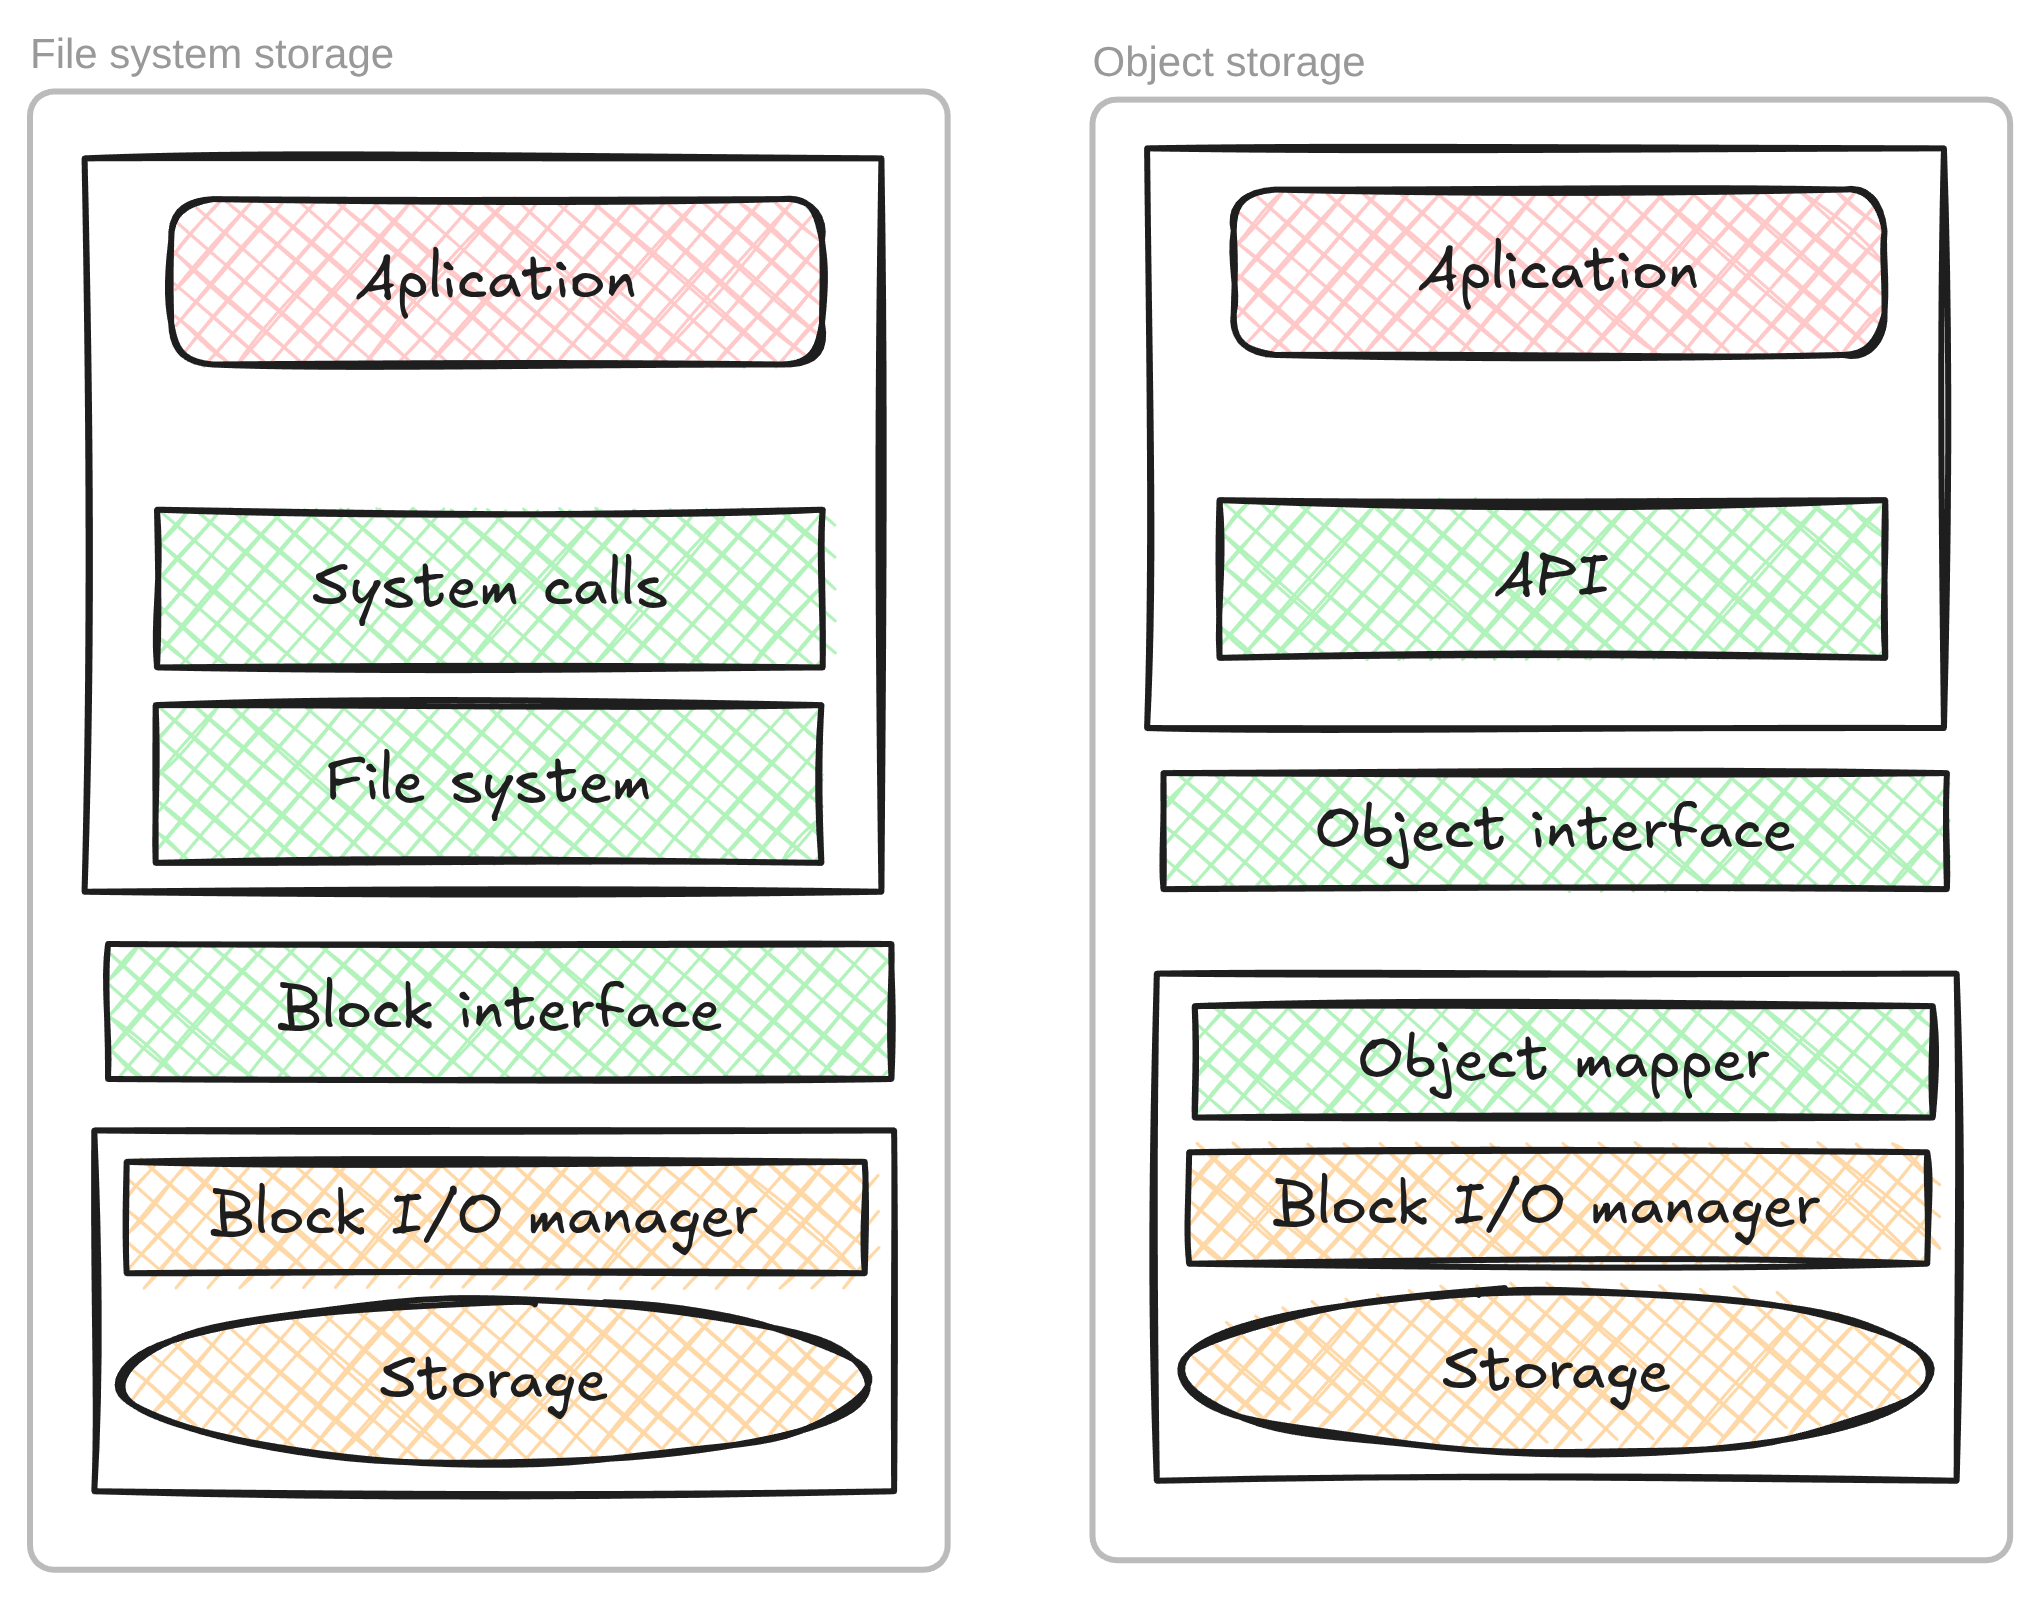
\includegraphics[width=0.9\textwidth]{images/object.png}
    \caption[Comparison  of storage interfaces]{
        \label{fig:object_storage_vs_fs}
        Storage interfaces for file systems and object storage solutions
        \cite{mesnier_storage_2003}
        }
\end{figure}

\vspace{1.5em}
The previous sections outlined three common abstraction layers and design patterns for storage systems. These abstractions remain fundamental to modern computing, and all following storage systems build on top of them.

\section{Software-Defined Storage}\label{ch:sds}
As many other fields in computer science (by both academic research and industrial needs) have evolved into new solutions, so has the storage subsystem. One of the directions storage subsystems went is towards distributed storage systems (its motivations and architecture will be discussed in the following chapters). Contemporary distributed storage solutions are frequently built within the broader framework of software-defined systems, specifically software-defined storage (SDStorage).

The software-defined system (SDSys) paradigm is a significant architectural shift whose main idea is to implement, through software, the management and control of underlying physical infrastructure. Such systems typically leverage existing hardware as a substrate, upon which software layers provide extended functionality and policy-driven behavior. \cite{moucha_software_2021, darabseh_sdstorage_2015}.

A core goal of any SDSys is to hide the complexity of resource management and control from end users \cite{darabseh_sdstorage_2015}. By moving resources to service-like abstractions, SDSys enables a clear expression of requirements (e.g., QoS levels, placement policies), consistent and system-wide enforcement of policies \cite{darabseh_sdstorage_2015, moucha_software_2021}. The first widely adopted realization of this idea appeared in networking as software-defined networking (SDN). Later, an experimental framework called SDStorage was introduced in an article presented by Staffordshire, IBM Corporation, and other co-authors, taking inspiration from the implementation of SDN (concretely Mininet Software) \cite{darabseh_sdstorage_2015}. The authors of the article mention that the SDN technology helped them create the foundation of SDStorage.

\subsection{SDStorage Architecture}
From a higher-level perspective, software-defined storage is typically split into two planes: a control plane and a data plane. The control plane provides the system’s intelligence. It maintains a global view of resources, translates API requests into executable rules and actions, orchestrates placement, controls replication, and monitors health and performance. The data plane executes those rules along with the I/O operations on the underlying physical storage system, serving as a data layer for the control plane. It performs the actual read/write operations. The control plane uses the data plane to enforce the policy (e.g., caching, compression, encryption, replication\ldots). This separation reduces complexity, improves modularity, and enables consistent policy-driven behavior across heterogeneous hardware. \cite{moucha_software_2021}

\begin{itemize}
    \item \textbf{Control Plane} \\
    The control plane is the core of an SDStorage architecture, providing the system’s intelligence and acting as its coordinating brain. It is typically implemented as a logically centralized controller that coordinates, manages, and enforces policies throughout the storage environment. Its primary functions include provisioning and orchestrating volumes, automating lifecycle operations, maintaining a global view of resources and state, and translating user-defined (business-level) policies into concrete executable instructions. Through the control plane, SDStorage platforms enforce QoS and other policy requirements consistently across heterogeneous backend (physical storage). \cite{darabseh_sdstorage_2015, macedo_survey_2021, faisal_software-defined_2024}
    \item \textbf{Data Plane} \\
    The data plane is where the storage service is realized -- it executes I/O against underlying physical storage. It is responsible for performance, durability, and efficiency. It is a component available to the control plane that enforces controller-defined policies over data. Among typical I/O functionality, it may be responsible for replication, compression, deduplication, and caching. Within SDStorage, the data plane corresponds to the underlying storage infrastructure and assets on which these operations are performed. \cite{darabseh_sdstorage_2015, macedo_survey_2021, faisal_software-defined_2024} \\
    Its main role is to abstract the underlying hardware storage (e.g., block and file systems) and provide it to the control plane as unified storage.
\end{itemize} 

The last component, not often mentioned in the SDStorage system, is the management layer. This component is usually responsible for organizing and managing the entire system and interacts with the control plane. It can be used to describe management tools (such as web user interfaces) to administer such systems \cite{kohli_next_2022, moucha_software_2021}. Since it is rarely explicitly discussed and often merged into the control plane, only data and control planes will be discussed in the thesis.

Together, the control plane and the data plane form a complete storage system capable of providing core storage functionality. The schema of such systems, with the corresponding responsibilities, is shown in figure \ref{fig:architecture_of_distributed_solutions}\footnote{Figure shows all three components (control, management, and data plane). Control and management planes are often merged into one component.}.

\begin{figure}[!ht]
    \centering
    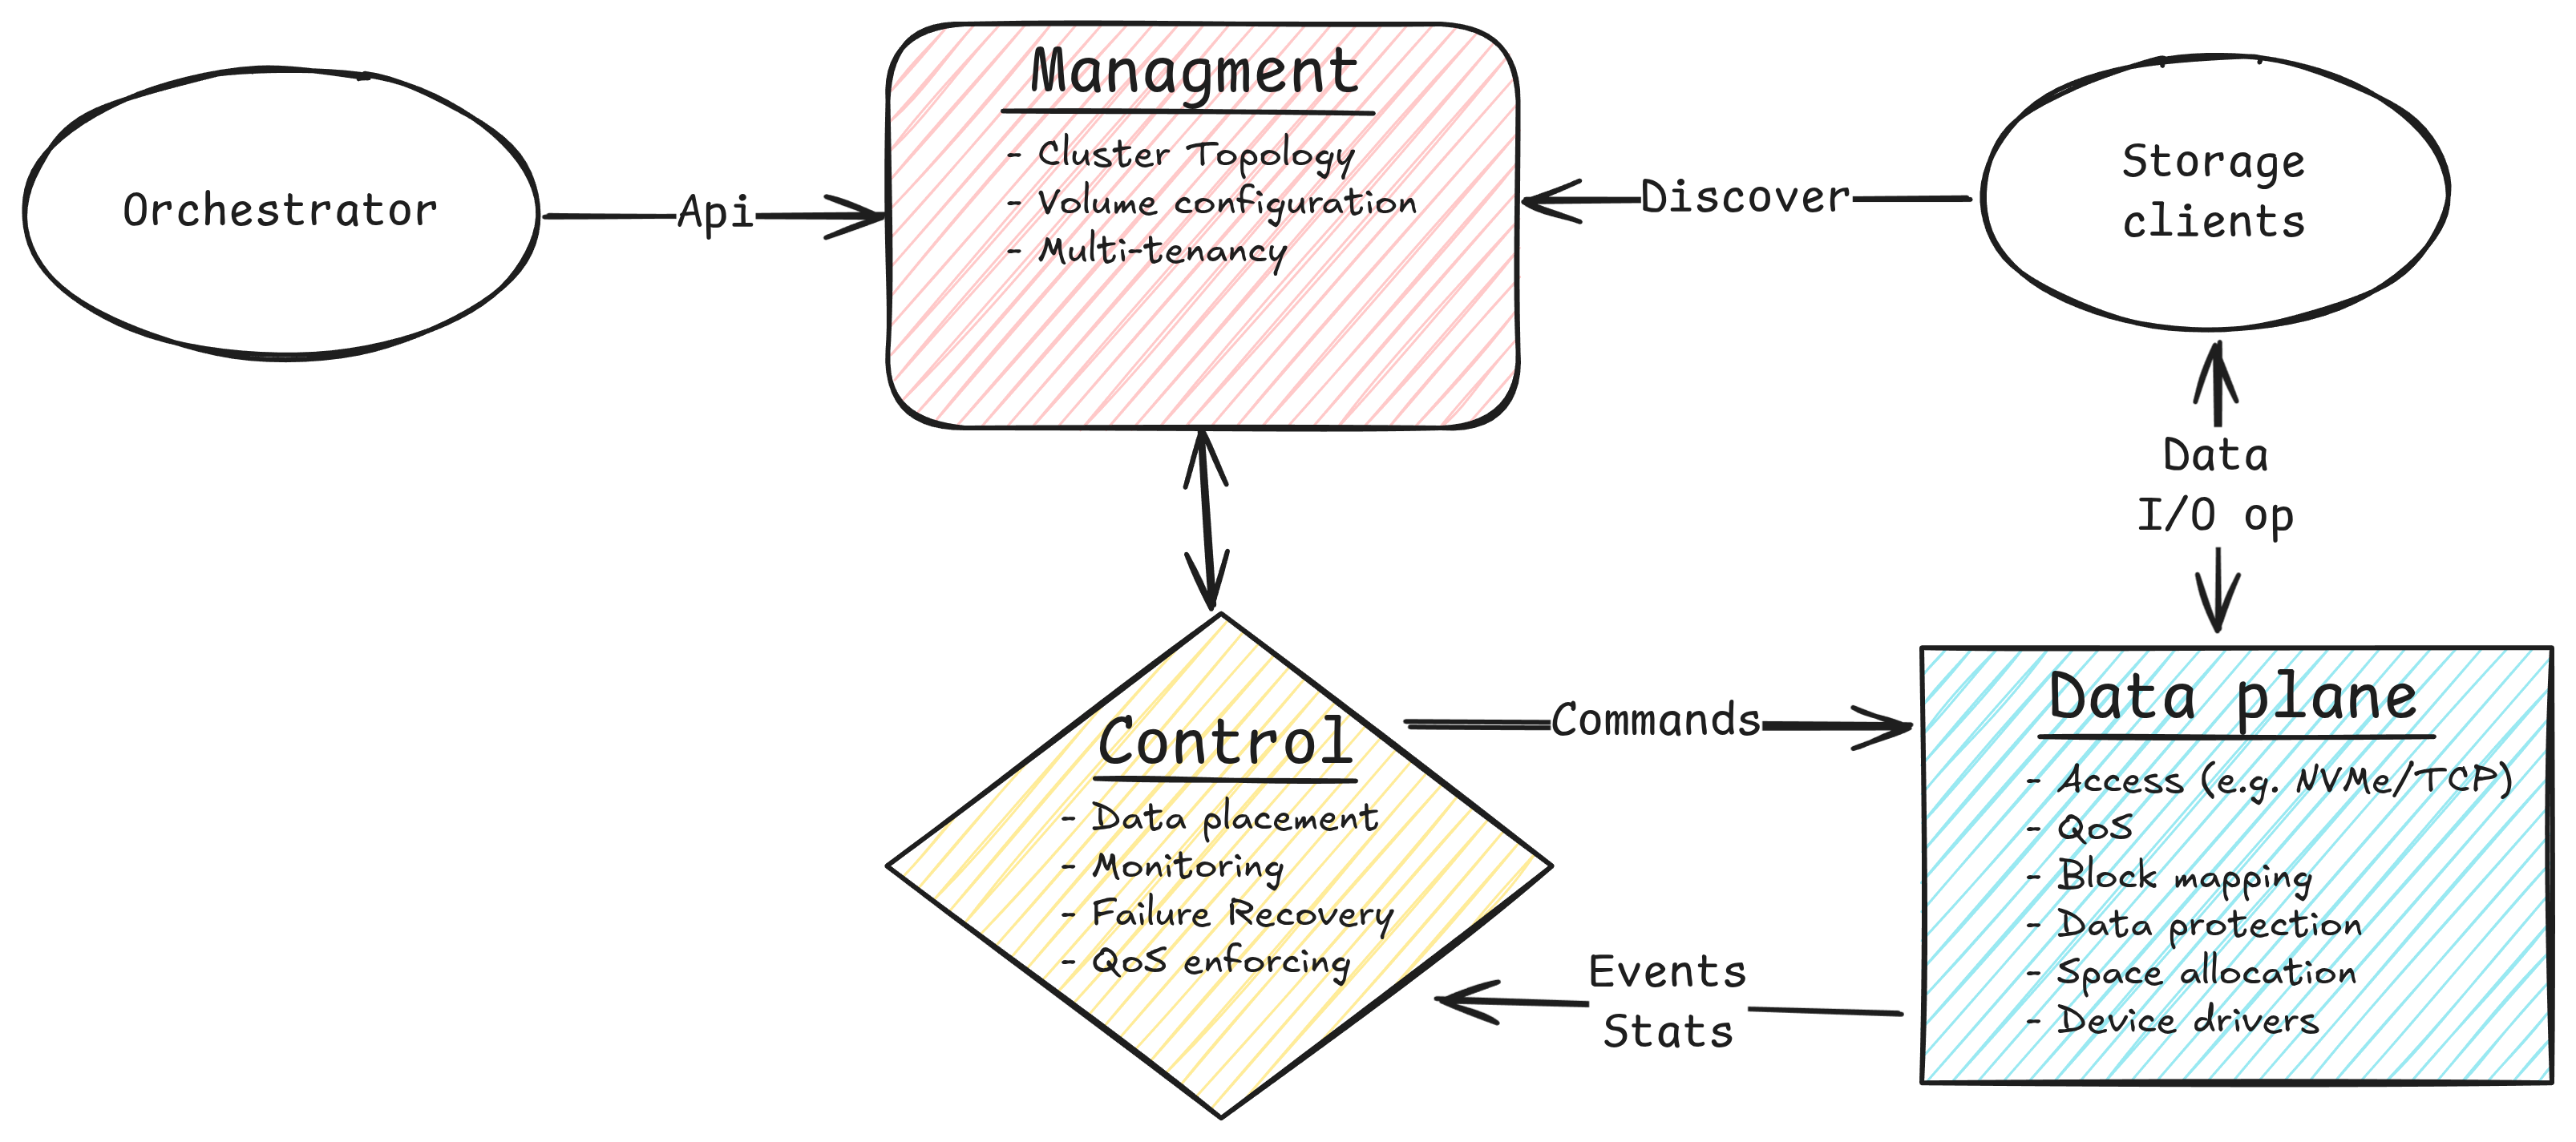
\includegraphics[width=0.9\textwidth]{images/architecture_of_distributed_solutions.png}
    \caption[Architecture of SDStorage]{
        \label{fig:architecture_of_distributed_solutions}
        Architecture of SDStorage\cite{kohli_next_2022}
        }
\end{figure}

\subsection{Interfaces on SDStorages}
Traditional storage provides an interface via the systemcalls implemented by the underlying operating system. In SDStorage, the control plane serves as the primary entry point for users and applications, offering explicit application interfaces (APIs) to interface with storage. This is the main difference between traditional systems. As in object storage (Figure \ref{fig:object_storage_vs_fs}), the SDStorage interface is a general API that offers greater control. This allows users to define any type of API suitable for the needs of a concrete storage system and its application needs.

By decoupling the data plane and control plane and freeing the storage stack from dependencies on a rigid interface, SDStorage makes the storage stack more flexible and extensible. It can compose new services, evolve semantics (e.g., tiering, encryption, erasure coding). It also enables modifying storage for specific needs without large changes to the API \cite{darabseh_sdstorage_2015}.

\subsection{Advantages of SDStorage}
Treating the storage system as software brings several benefits by rethinking the schema in a software-oriented way. The following are some advantages of using SDStorage:

\begin{itemize}
    \item \textbf{Removes Hardware Dependency} \\
    Software-defined systems (in general) decouple functionality from underlying hardware. This enables organizations to deploy applications on mixed-vendor infrastructure. Hardware independence reduces dependence on specialized appliances and vendor lock-in. This leads to a more flexible deployment environment and may reduce the overall system cost. \cite{faisal_software-defined_2024}
    
    \item \textbf{Performance Scalability} \\
    The architecture design of SDSys brings scale-out nature even to SDStorage systems. Storage resources can be expanded horizontally by adding new data nodes, without disruptive architectural changes. This allows capacity and I/O performance to grow and scale out. Some solutions claim even the possibility to scale out linearly (when pre-requisistes) are met. \cite{parkes_cephio_2025}

    In addition to data scalability, the software way of thinking allows easy implementation of cache subsystems at any specific abstraction level. This allows tuning performance for specific needs. It is suited for high-performance environments with the possibility of tuning parameters such as latency, file sizes, and consistency \cite{faisal_software-defined_2024}.
    
    \item \textbf{Operations, Automation, and IaC} \\
    SDSys replaces device-centric management with a centralized control plane that controls heterogeneous resources. Administrators can manage diverse pools of infrastructure from a single logical point, using uniform policies instead of device-specific configuration. This unification significantly reduces operational complexity and human error.

    By introducing the management plane, the operations of storage systems can be easily abstracted by policies and other concepts. Provisioning, data placement, replication, backup, and lifecycle operations are expressed as high-level policies and executed automatically by the control plane.
    
     API-driven programmability makes infrastructure fully scriptable and allows use of Infrastructure-as-Code practices. \cite{faisal_software-defined_2024}
    \item \textbf{Data and Resource Management} \\
    SDStorage introduces a unified approach to managing heterogeneous storage resources without limiting their specific usage. By providing a unified view across block, file, and object storage, it enables consistent monitoring, policy enforcement, and capacity planning across diverse media types. \cite{faisal_software-defined_2024}

\end{itemize}



\section{Distributed Storage Solutions}\label{sec:distributed_solutions}
The previous Chapter \ref{ch:sds} has highlighted that software-defined storage solutions have a crucial role in designing distributed storage solutions. Distributed storage solutions represent another approach to address the continuously evolving needs of storage systems.

Modern computing environments face significant challenges in managing the growing volume of data. Traditional storage solutions often struggle to meet the scalability, fault tolerance, and high-performance requirements of modern applications. The rise of cloud computing has amplified these challenges, as dynamic workloads and distributed applications demand storage solutions that can adapt and scale efficiently. Another part of computation that introduces new challenges for storage systems is grid computing, in which parallel access to storage is required. \cite{langr_paralelni_2024}

The concept of distributed storage solutions has emerged to address these issues. A distributed storage solution can represent various solutions or their combination. To clarify the solutions, here is a list with explanations.

\begin{itemize}
    \item \textbf{Parallel File and Object Writing} \\
    Traditional file systems and object stores do not allow parallel writes to the same file or object at the same time. When two subjects attempt to access (write) the data simultaneously, they must synchronize their access. This can be a problem in HPC, when data are usually enormous and computational power is time-limited. Distributed storage solutions address this by enabling parallel writes to different data nodes in a cluster. \cite{langr_paralelni_2024}
    \item \textbf{Replicated Storage} \\
    Replicated storage ensures data redundancy by storing multiple copies of the same data across different nodes in a distributed system. This improves data reliability and availability. If one node fails, the system can seamlessly access data from another replica. Replication can be synchronous (immediate replication to all nodes) or asynchronous (updates occur after a delay). Common use cases include disaster recovery, fault tolerance, and read-intensive workloads, in which replicas distribute the read load. \cite{tudelft_225_2023}
    \item \textbf{Remote Storage} \\
    Remote storage allows data to be stored on a different physical or virtual location and accessed over a network. It decouples storage from compute resources, enabling greater flexibility in resource allocation. Network protocols such as NFS (Network File System) or iSCSI (Internet Small Computer Systems Interface) facilitate access to remote storage. This approach is often used in cloud environments and distributed systems where centralized data storage is necessary. \cite{vondra_storage_2022}
    \item \textbf{Remote Storage Pools} \\
    Remote storage pools aggregate multiple remote storage resources into a single logical pool. This abstraction allows users to manage and utilize storage more efficiently without worrying about the underlying physical location of the data. Storage pools can span multiple nodes, data centers, or even cloud regions, offering seamless scalability, load balancing, and high availability. This is particularly useful in hybrid and multi-cloud setups. \cite{vondra_storage_2022}
\end{itemize}

\vspace{1.5em}
From now on, this thesis will mainly discuss remote storage pools. When addressing distributed storage, consider a solution that can serve remote storage pools. This chapter will focus on the scalability of those storage systems, their replication, fault tolerance, performance, and the APIs they offer to users. Other types of distributed storage are not relevant to this topic.

\subsection{Architecture of Distributed Storages}
The architecture of modern distributed storage solutions is highly dependent on the principles of Software-Defined Storage established in Chapter \ref{ch:sds}. While traditional storage architectures tightly bind data to specific hardware controllers, distributed solutions leverage SDS decoupling of the control and data planes to offer storage that spans multiple servers (nodes), creating a unified system.

In a distributed SDStorage architecture, the control plane usually maintains a map of the cluster (set of nodes) and controls the data plane on each node. It uses the raw storage capacity provided by the data plane's individual nodes into a shared, logical construct often referred to as a Storage Pool.

Instead of interacting with physical disks, the control plane abstracts these resources. It treats the collection of all underlying drives in the network as a single contiguous storage space. This architecture extends the SDStorage's features to distributed systems and adds several others. The key ones are:

\begin{itemize}
    \item \textbf{Global Resource Management}  \\
    The control plane maintains the global state of the storage cluster. It usually monitors the total available capacity and health of the pool, and the state of the data node. This makes it easier to maintain a storage pool as a single coherent system rather than managing individual nodes in isolation.
    \item \textbf{Dynamic Scalability} \\
    Data nodes in distributed storage systems are treated as "worker" nodes, controlled by the master (control plane). Data planes can be independent of each other, since they just serve resources to the control plane. This allows easy dynamic scaling. When a new node is added to the cluster, the control plane detects the new data plane resources and automatically adds them to the storage pool, increasing the total capacity without service interruption.
    \item \textbf{Policy-Based Distribution} \\
    In a distributed environment, data placement and resource allocation are controlled by the control plane. This allows organizing data by logical definitions rather than hardware ones. This adds the possibility of implementing various data placement optimizations for any required use cases.  This enables the enforcement of Quality of Service rules. An example of QoS could be fault tolerance or throughput limits.
\end{itemize}
\cite{mark_carlson_software_2015, macedo_survey_2021, moucha_software_2021}

% TODO refraze
Another key advantage of distributed storage solutions is the ability to load-balance client requests across multiple data planes. Because data are typically replicated across several nodes, the system can direct read requests to any node that currently holds the requested data. This improves throughput and increases resilience to transient performance degradation of individual nodes. The concrete mechanisms for request distribution depend heavily on the particular implementation; therefore, it will be discussed for each storage system as it is introduced in the following text. \cite{macedo_survey_2021, moucha_software_2021}

\vspace{1.5em}

By combining the capabilities of software-defined storage and applying them to distributed storage systems, it's possible to create storage systems composed of multiple nodes that form a storage pool. With decoupling data storage layer and control layer, it is potential to build storage suitable for various needs. 

Once physical resources are aggregated into a pool, the system can carve out logical units for consumption, whether as block devices (volumes), file systems, or objects collections. Users and applications then interact only with needed logical units, while the system fully abstracts away the physical layout of the data. This architecture directly fulfills the main requirement of \emph{remote storage pools} discussed in the previous section. \cite{macedo_survey_2021, moucha_software_2021}

This architecture offers a wide range of possibilities when designing storage systems with defined QoS, based on their needs. The above-listed advantages come with trade-offs and problems that those systems need to address, the most common of which are data durability, consistency, and trade-offs among consistency, availability, and failure resilience.


\subsubsection{Data Durability}
Data durability describes the ability of a storage system to store data in a way that is resilient even for partial failures. In distributed storage, durability is primarily about ensuring that the data can survive hardware failures, software bugs, and operational mistakes without permanent loss. Because modern systems store large volumes of data on commodity hardware and across many nodes, failures are expected rather than exceptional, and durability mechanisms become a core part of system design.

In practice, durability is achieved by introducing redundancy and recovery plans. Two common approaches can be distinguished by their recovery characteristics. The first approach is backup, which typically provides durable copies at a lower operational cost but with slower recovery. The second approach provides fast recovery through online redundancy, such as replication or sharding combined with redundancy, in which the system can continue serving data even when some components fail and automatically rebuild missing replicas/shards.

This text will focus on online redundancy, since it's specified as one of requirements for solving problem described in the beginning of the thesis.  
\paragraph{Replication} \mbox{} \\
One way to ensure data durability is to replicate the data. That means keeping a full copy of the data on multiple nodes. This is one of the easiest and most intuitive ways to implement data durability. By maintaining data replicated on various nodes, it is guaranteed that no data will be lost in any case of failure in which at least one copy of the remaining data is available. The advantages of replication are its simplicity, which makes it easy to design recovery plans in case of any failure and partial (copy) data loss. Creating a copy of the data and replicating it across multiple availability zones also introduces the possibility of load-balancing read requests across data locations.\cite{kleppmann_designing_2017, liu_evaluation_2018}

An example of a replication solution is the Distributed Replicated Storage System (DRBD). DRBD is an open-source solution for block replication over the network between multiple Linux storage nodes. Linbit developed it, now DRBD is one of the most common solutions for block replication across Linux servers. Although there are other solutions, DRBD is one of the most used. It is mentioned here as a concrete implementation.

DRBD is implemented as a kernel module in a Linux kernel. It enables reliable replication (RAID 1) for Linux nodes across a network. This replication is often used to meet requirements for fault tolerance and high availability systems. Thanks to the replication, when all nodes but one are unavailable, the remaining one can still offer a fail-over and serve its purpose. This replication comes with a network usage cost and more storage space consumption from the storage pool. \cite{linbit_drbd9_2025}

Even though DRBD itself does not implement a distributed storage system (storage pool based) it's often used as a part of solutions to those systems as you will see in Section \ref{sec:linstore}

\paragraph{Partitioning} \mbox{} \\
Another approach used for data durability and fault tolerance in distributed storage is \emph{partitioning}. Partitioning (also called \emph{sharding}) splits the stored object into multiple smaller pieces (partitions) and distributes them across different nodes in a storage pool. By itself, partitioning mainly changes placement of the data. To add data durability it is often combined with additional redundant information to offer failure recovery (e.g., parity data), such data enables recovery in case of failure. In such a design, the system stores only a subset of redundant fragments instead of a full copy, so data can remain readable and recoverable even after a node outage. \cite{purestorage_what_2025}

This method is much more space-efficient than replication since it does not have to store full replication data. The disadvantage of this approach is a performance cost when data are being restored or written since partitions need to be recalculated. \cite{purestorage_what_2025} This type of durability mechanism is often better for cold data, which is not often accessed and modified.

In storage systems, the mechanism that turns partitioning into a durability method is commonly \emph{erasure coding}. Erasure coding encodes data into $k$ data fragments plus $m$ parity fragments (often marked as a $(k+m)$ scheme), distributed across different nodes. Such system allows data to be reconstructed from \emph{any} $k$ out of the $(k+m)$ fragments. This provides fault tolerance with substantially lower storage overhead than full replication, at the cost of additional computation during writes and recovery. \cite{simplyblock_authors_erasure_2026} To better understand mechanism of erasure coding, see Figure \ref{fig:ec}.
% TODo show n picture
\begin{figure}[h!t]
    \centering
    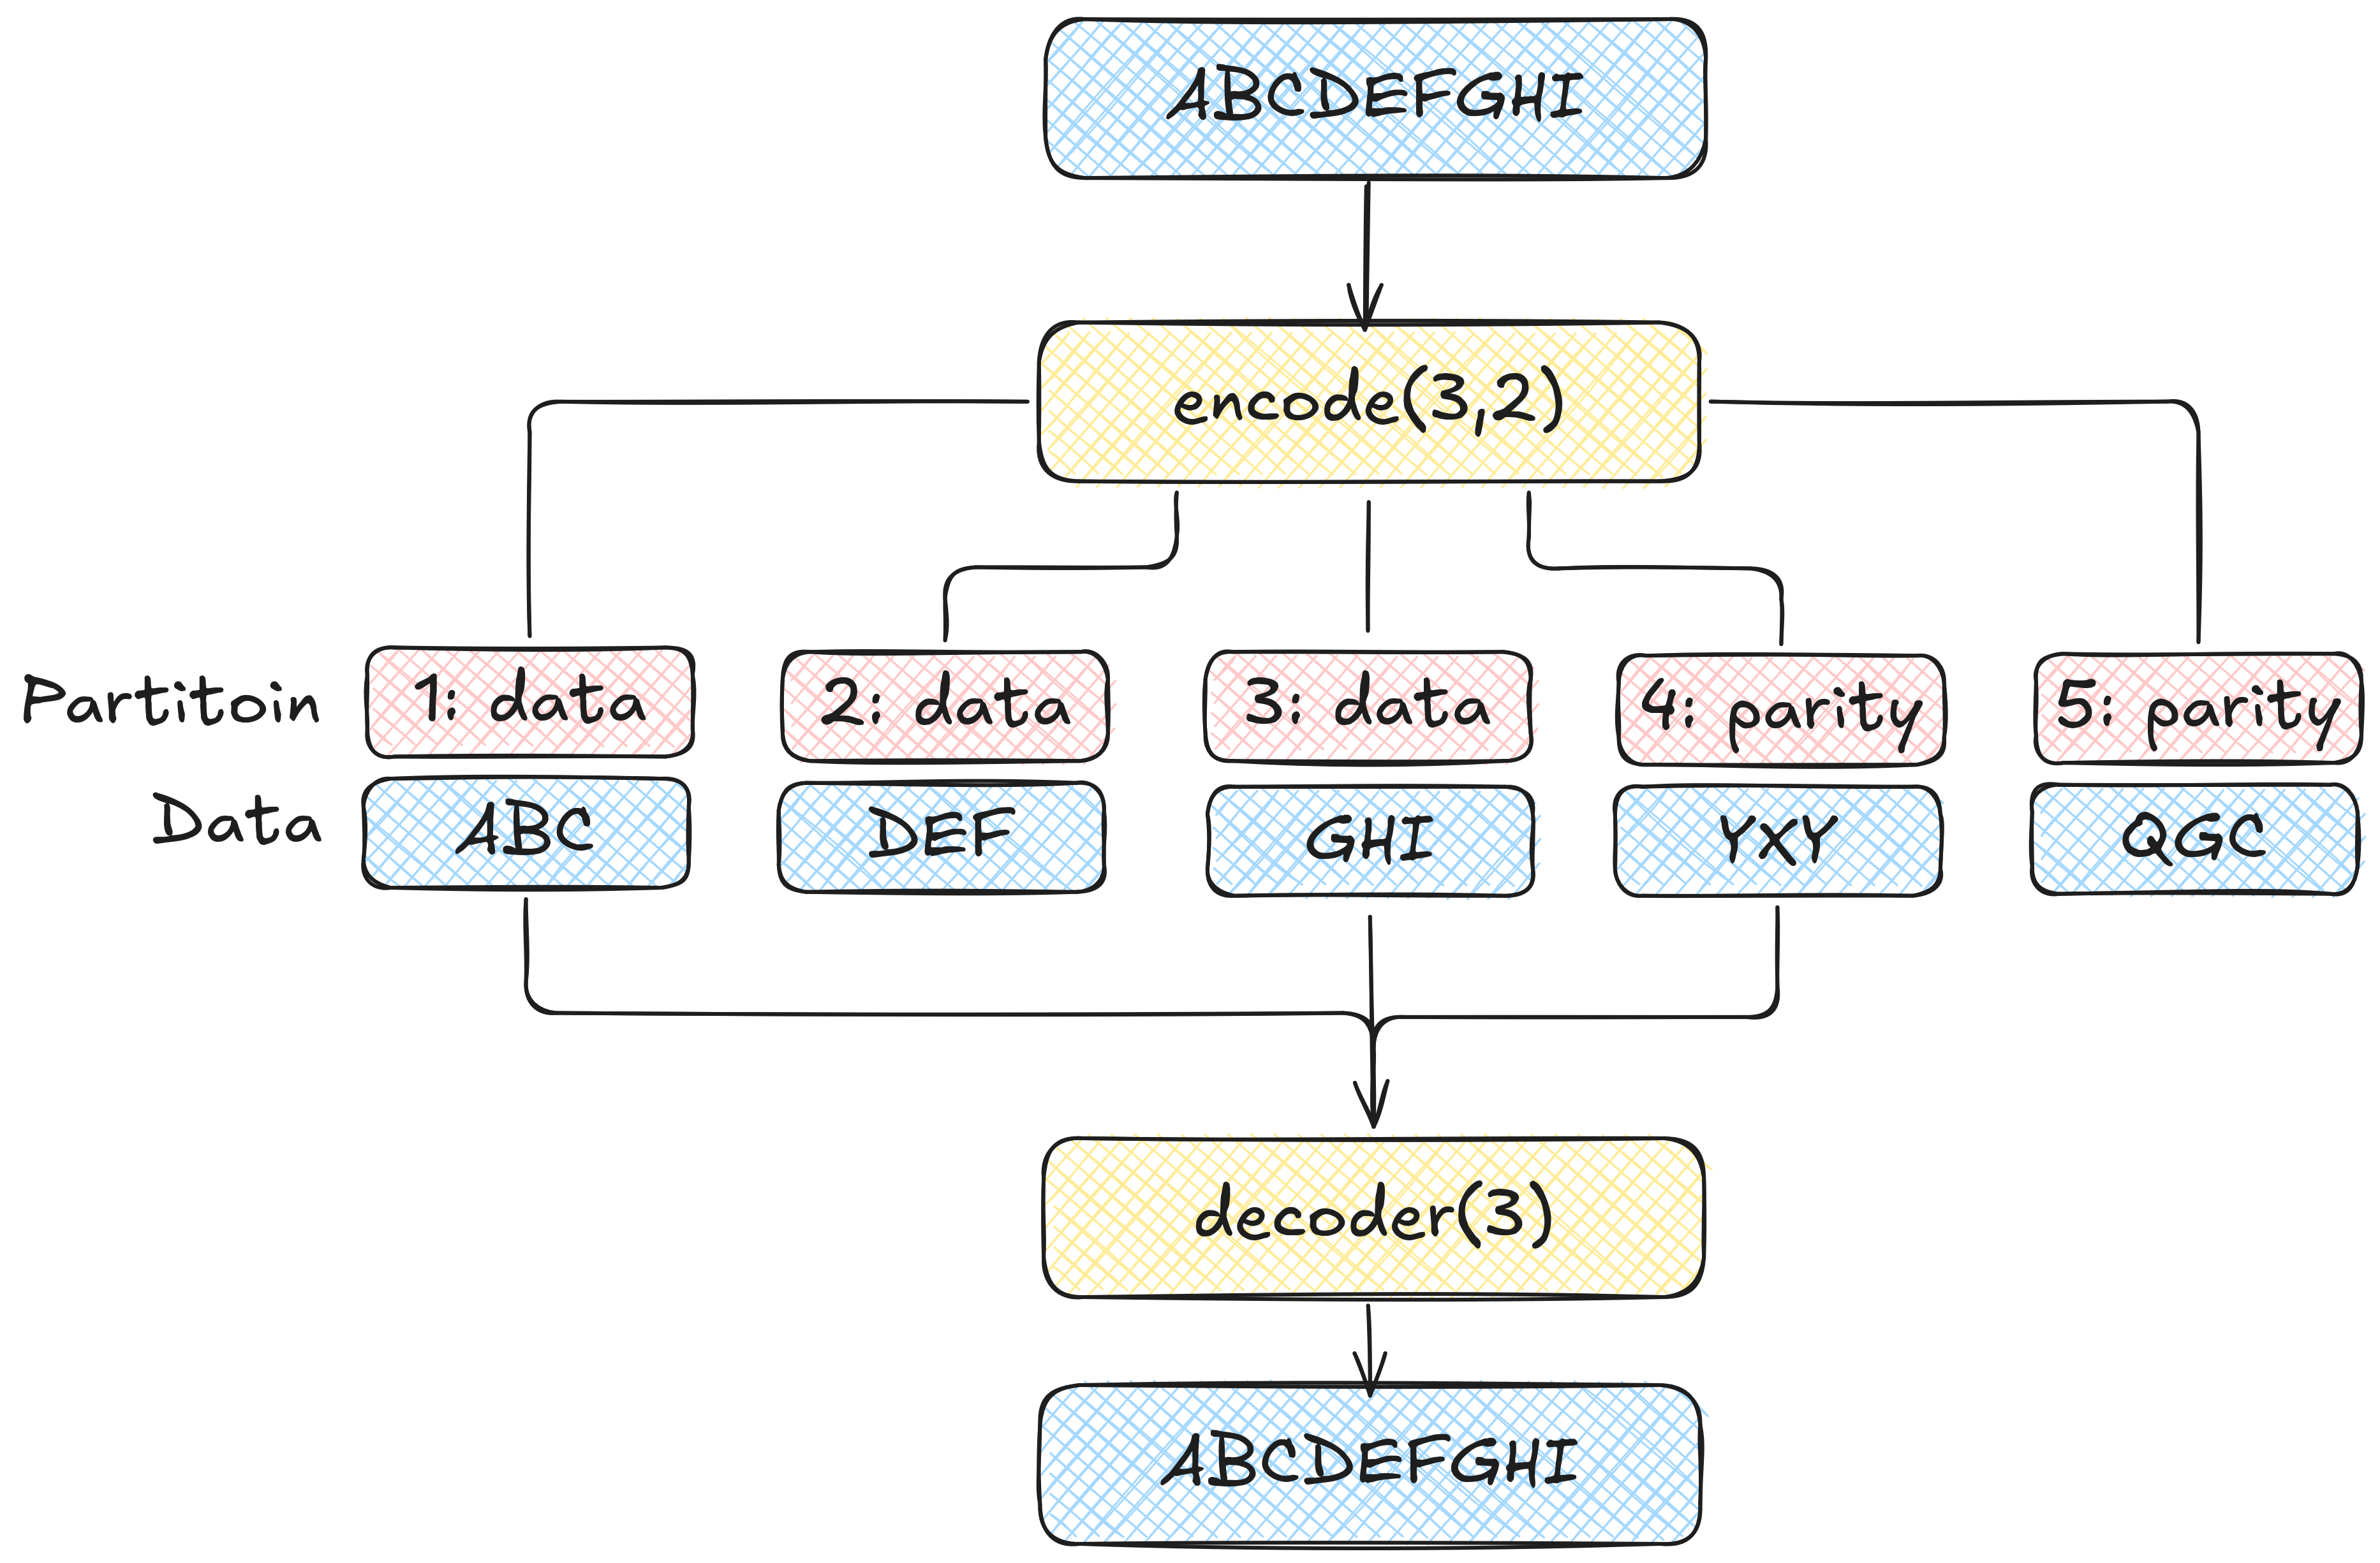
\includegraphics[width=0.9\textwidth]{images/ec.png}
    \caption[Erasure-coding schema]{\label{fig:ec}Erasure-coding schema -- $(3, 2)$\cite{ceph_authors_erasure_2016}}
\end{figure}
\vspace{1.5em}

% TODO the partitionng is often combined with replicatoin
\subsubsection{Consistency}
Introducing distributed systems that care about data durability, high availability, etc., always comes with shared data or knowledge of the system. Such systems must ensure the consistency of shared data. In a distributed system that contains data shared among servers, all nodes have a unique view of the data. It is critical to ensure that data stored on a distributed system remain accurate and coherent across all nodes. In storage systems, there are two main consistency patterns that describe how consistent the data are in a distributed system.\cite{geeksforgeeks_consistency_2025}

\begin{itemize}
    \item \textbf{Strong Consistency} \\
    \enquote{\textit{Ensures that all nodes in the system have the most up-to-date data at all times, with no lag or inconsistency between replicas.}}\cite{geeksforgeeks_consistency_2025}
    \item \textbf{Eventual Consistency} \\
    \enquote{\textit{Allows for temporary inconsistencies between replicas but guarantees that they will eventually converge to a consistent state without intervention.}}\cite{geeksforgeeks_consistency_2025}
\end{itemize}

Consistency levels are an important property of any distributed system that contains data for several reasons. Since distributed solutions are designed to enable scalability and prevent failures such as node outages, it is important to specify what happens in the event of data loss. Consistency patterns describe how systems behave in adverse scenarios and which states can or cannot guarantee correct data integrity. Among data integrity consistency patterns, ensuring quality of service of distributed solutions may offer better performance optimizations.

There are many types of consistency, which typically lie between two main types. First one is eventual consistency.
It requires that any comparable events must be performed in ordered, meaning that any event that directly or indirectly operates on the same data must be evaluated in the same order on every node. This type of consistency ensures that events can depend on one another and are executed correctly (an object's modification will be performed only after it is created). This pattern ensures that the sequence of (correct) operations on data in a distributed system will be correctly executed on every node. \cite{kleppmann_designing_2017} Such ordering implies that the system will eventually reach full consistency for each operation. This means that for each operation, there exists (or will exist) a time at which this operation was performed on all available nodes in the distributed system, and at that point, all systems had a consistent set of data. This ensures that the entire global system will not diverge, but actively tries to reach the same state. It does not guarantee that such a state will appear on every machine at the same global time or at any time at all.  \cite{kleppmann_designing_2017}

The most restrictive type of consistency is strong. This type of consistency guarantees that at any time (global), all nodes that are part of the distributed system have the same data and are fully synchronized. This pattern keeps the data most secure, but severely limits the system's availability. The relation of consistency and availability is known as the CAP theorem.  \cite{kleppmann_designing_2017, jepsen_authors_consistency_2025}
\subsubsection{CAP and PACELC}
The above section described important properties of distributed storage systems. One of the motivations for distributed solutions is availability, which is another property common to such systems. The "ideal" system (among other properties) often aims for the highest availability, the strongest consistency, and the strongest durability. Such a system that maximizes all 3 properties cannot exist; this statement is known as the CAP theorem, introduced by Eric Brewer at the University of California, Berkeley.\cite{brewer_cap_2012}

The CAP theorem combines 3 properties (namely, C, A, and P) of a distributed storage system. C stands for strong consistency (having a single latest copy of the data). A stands for high availability, meaning the ability to serve any type of request without unnecessary delay. Lastly, P stands for partition network tolerance. Partition network tolerance means that the distributed system continues to operate even in the presence of network failures that partition it into isolated groups.

The CAP theorem says that any distributed system cannot fully satisfy all three properties and that it can only maximally satisfy any two properties. The reason for such a theorem is that any 2 properties will always disqualify the third one. To guarantee both consistency and availability, the system must guarantee that the network never fails. To maintain consistency in the presence of a partitioned system, the system must stop serving requests that would lead to inconsistent data. Lastly, to remain available during a partition, the system must allow nodes to continue processing requests even if they cannot communicate with each other, which may break consistency. CAP theorem is often displayed as a triangle in which only one edge can be satisfied (see Figure \ref{fig:cap}). \cite{brewer_cap_2012, abadi_cap_2012}

\begin{figure}[h!t]
    \centering
    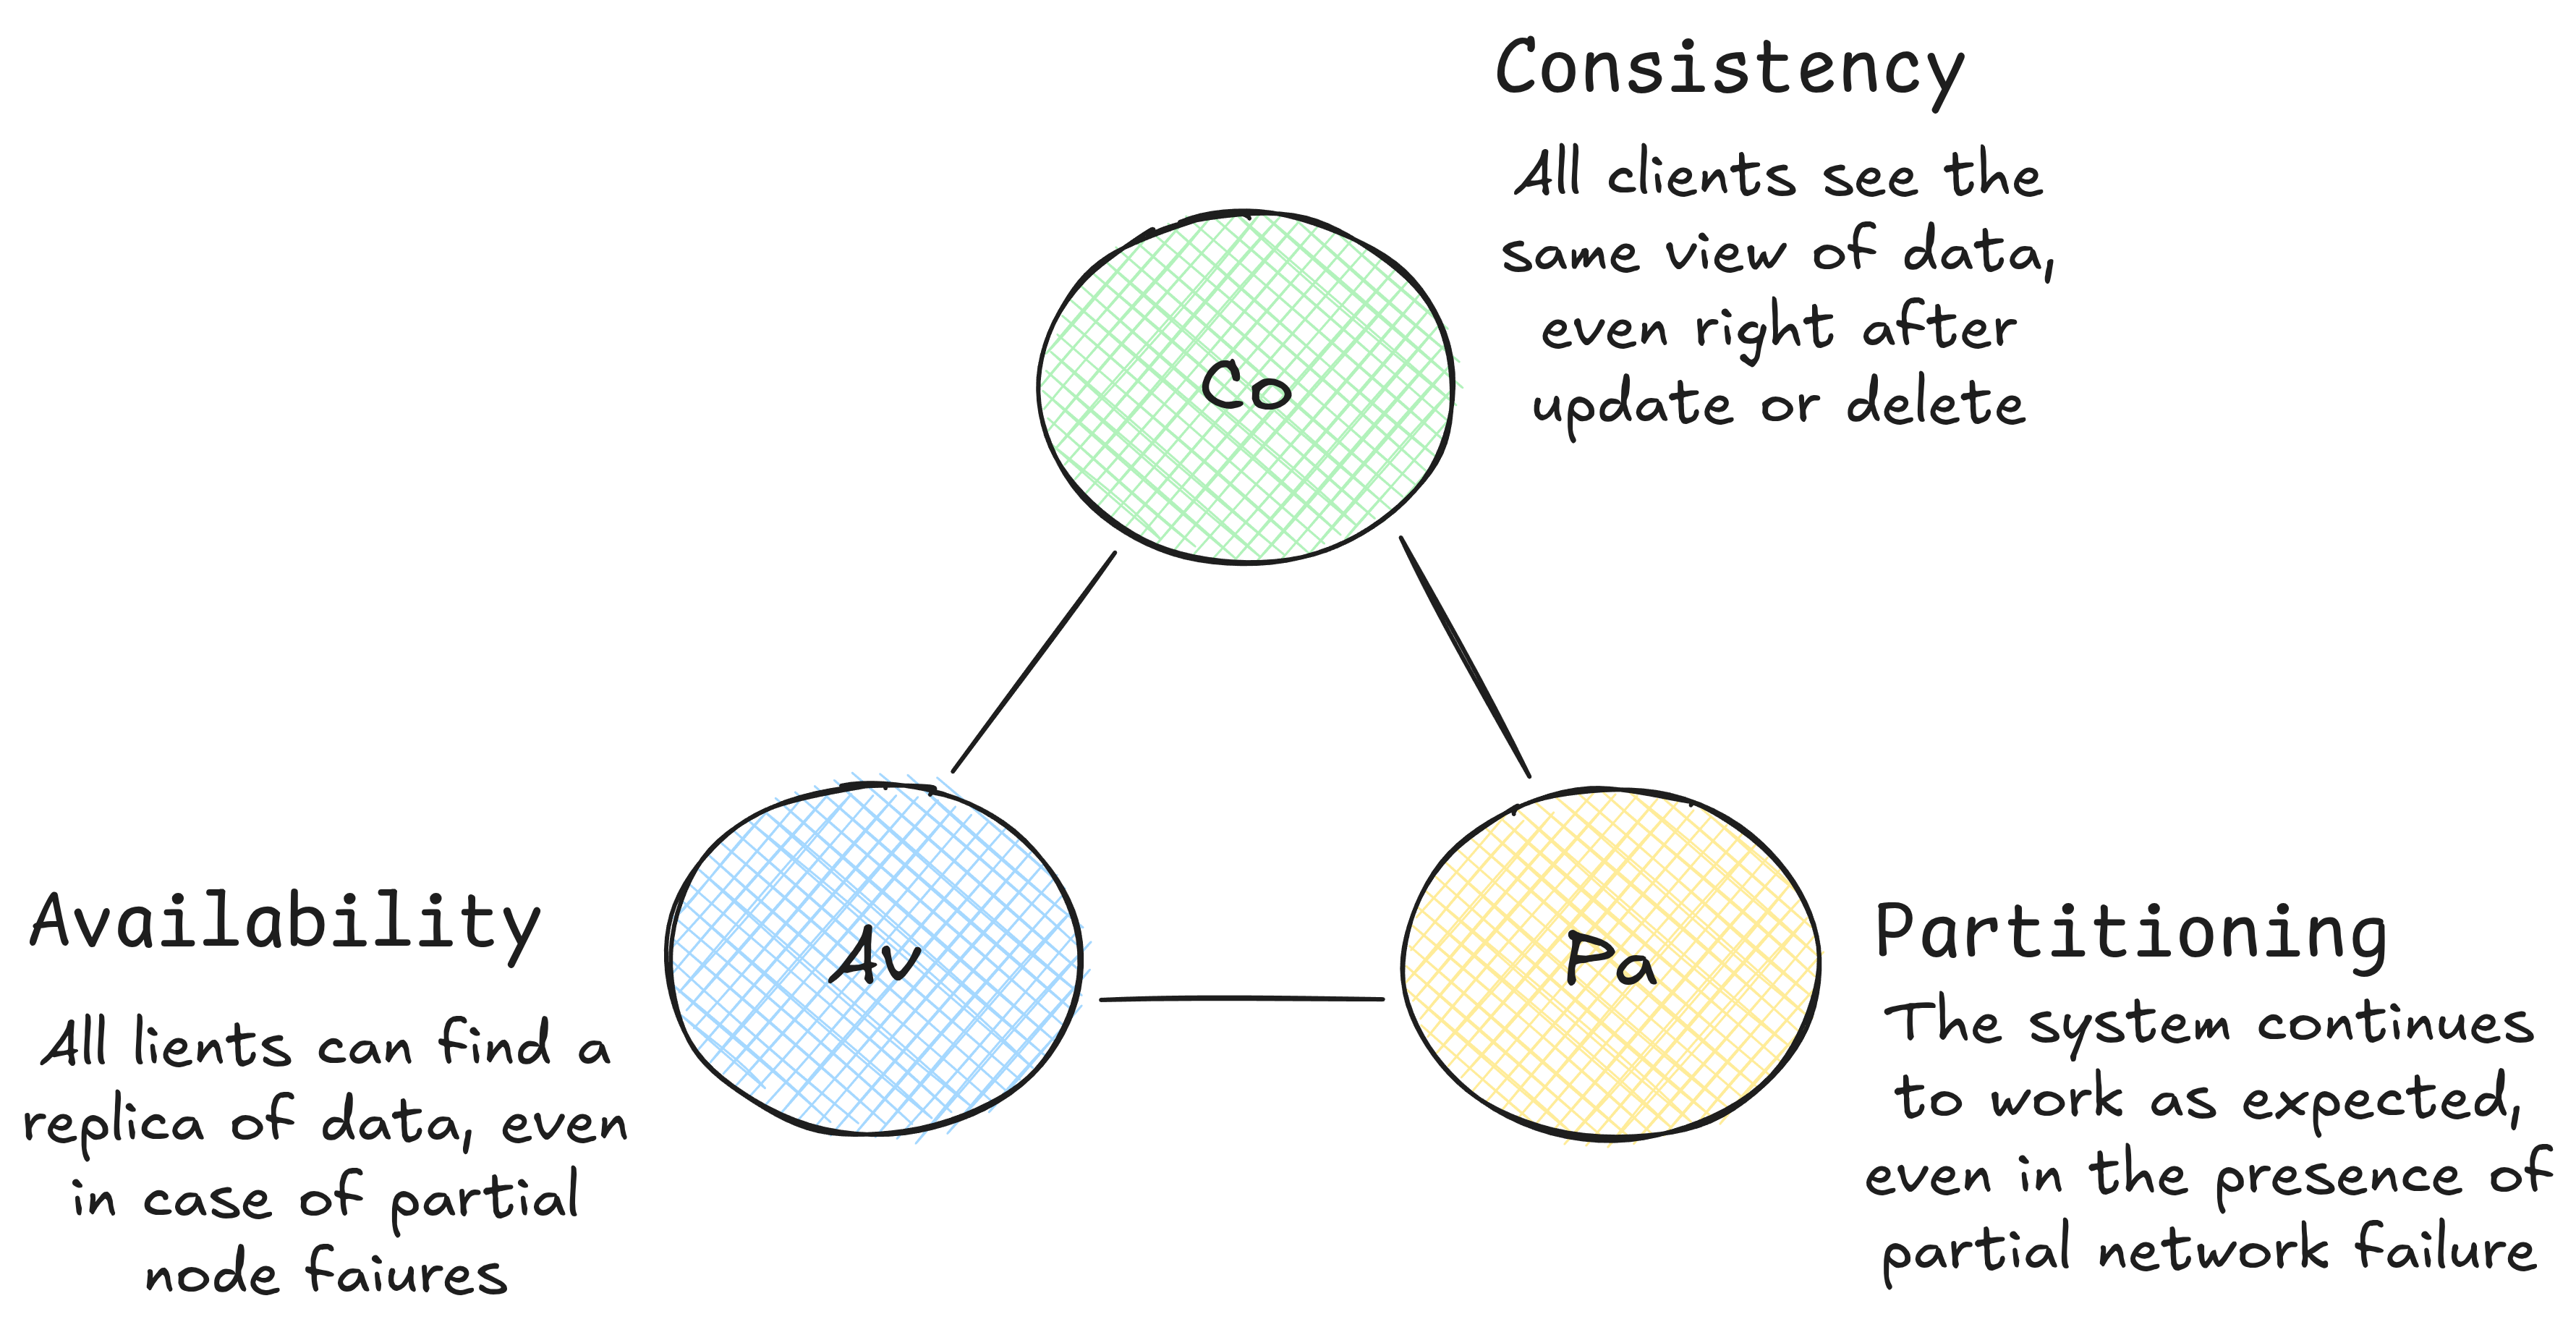
\includegraphics[width=0.9\textwidth]{images/cap.png}
    \caption[CAP theorem visualization]{\label{fig:cap}CAP theorem visualization\cite{medhat_understanding_2021}}
\end{figure}

CAP theory only describes the situation during network partitioning, which may occur in a distributed system, but it says nothing about the state in which the system is acting as a single, unpartitioned system. In such a case, the CAP theorem is extended to the so-called PACELC theorem. The PACELC theorem extends the CAP theorem (PAC) by adding the trade-off between latency and consistency (LC) even when the system is operating normally.If the system is not partitioned, it can serve only two out of three properties: latency, consistency, and availability. The logic rules behind latency, availability, and consistency are the same as in the CAP theorem. Its logic is visualized in Figure \ref{fig:pacelc}. \cite{geeksforgeeks_pacelc_nodate}

\begin{figure}[h!t]
    \centering
    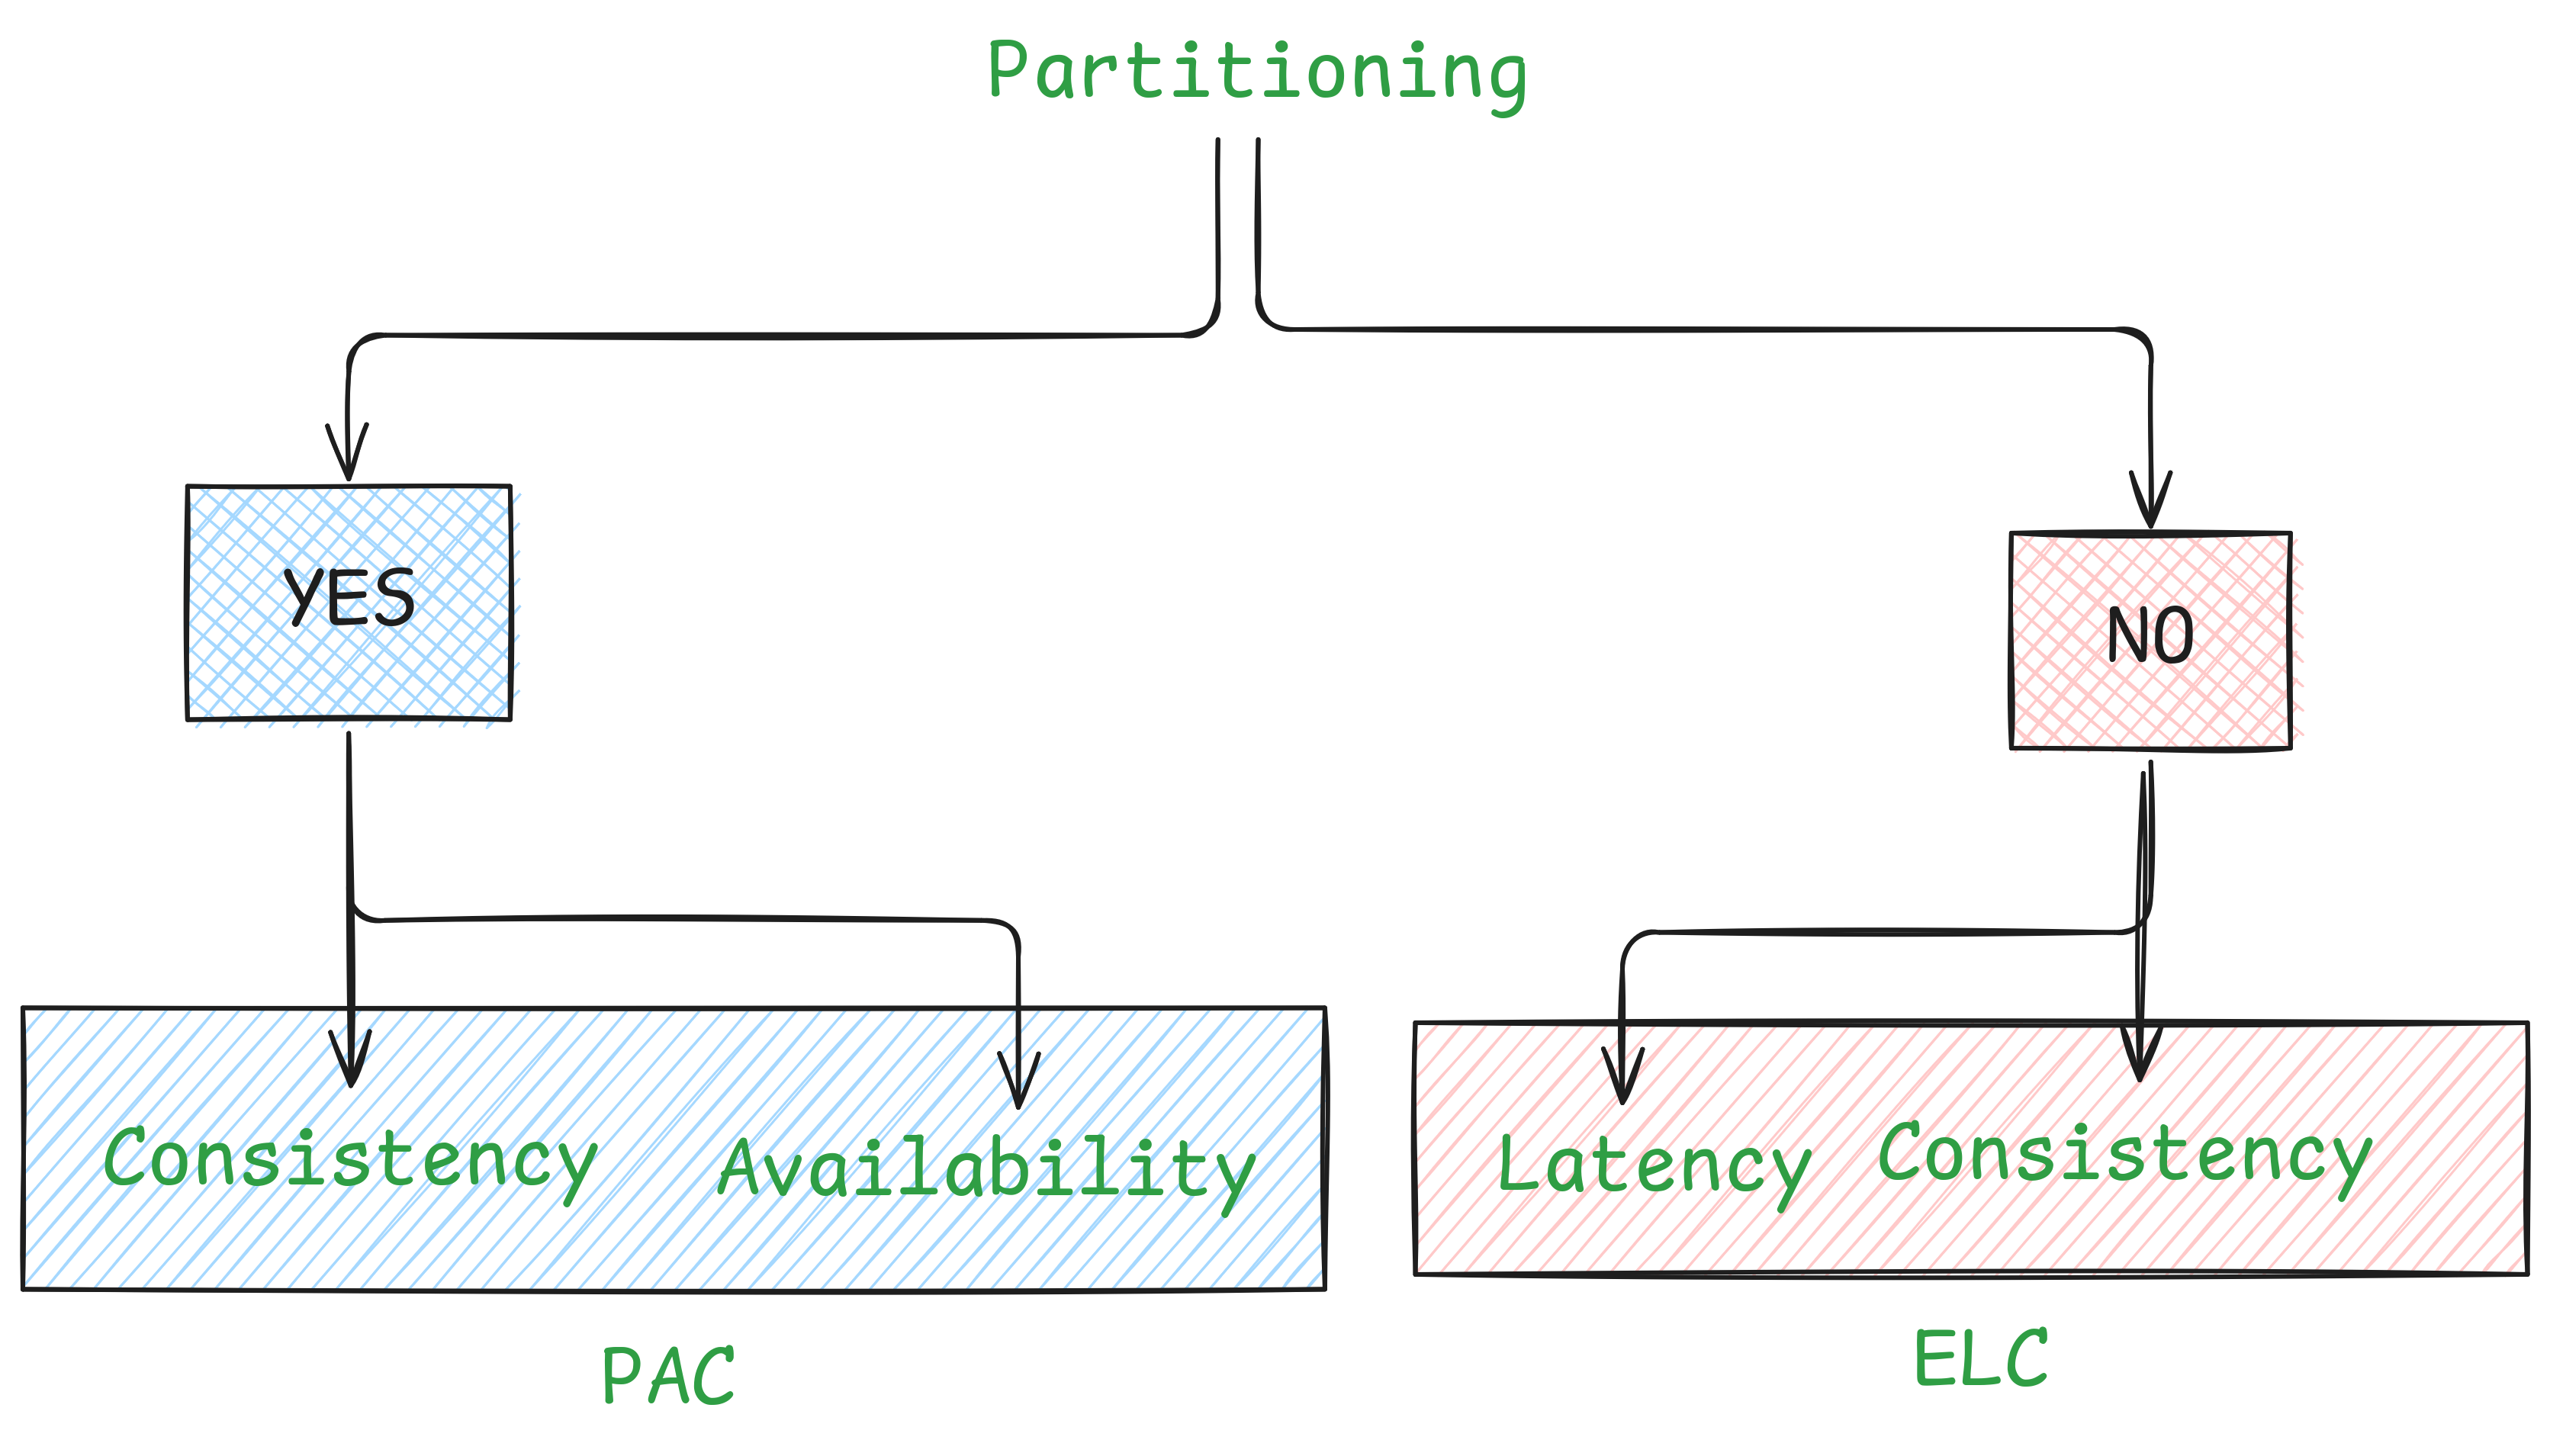
\includegraphics[width=0.9\textwidth]{images/pacelc.png}
    \caption[PACELC theorem visualization]{\label{fig:pacelc}PACELC theorem visualization (PAC, ELC)\cite{geeksforgeeks_pacelc_nodate}}
\end{figure}

\vspace{1.5em}

\subsection{Implementations of Distributed Storages}\label{sec:dfs_implementations}
\subsubsection{Ceph}\label{sec:ceph}
One of the most widely adopted scale-out storage systems is Ceph. It was originally created as a dissertation project by Sage Weil at the University of California, Santa Cruz. Today, the project is maintained by major corporations, most notably Red Hat \cite{vondra_storage_2022}. Ceph is commonly deployed as software-defined storage, approximately 75\%\cite{openstack_team_openstack_2025} of OpenStack installations (as of 2024) uses Ceph as its storage solution. It is also common choice for storage solution for Kubernetes environments. It provides a unified platform for all three primary storage abstractions: file system, object storage, and block storage. These interfaces are accessible via various APIs and protocols, including S3, iSCSI, NFS, and CSI.

The architecture of Ceph is built upon the RADOS system and the CRUSH algorithm. RADOS (Reliable Autonomic Distributed Object Store) provides an object store. The entire Ceph system operates on top of RADOS, where data are striped across RADOS objects \cite{cubefs_authors_cubefs_nodate}.

The fundamental atomic unit within RADOS is the object -- identified by a unique ID. These objects are isolated from each other and can vary in size. The object store organizes these objects into pools -- logical collections that define specific storage policies, such as the replication factor or geolocation constraints. 

The data plane of Ceph (and RADOS) is the OSD (Object Storage Daemon). An OSD is a daemon process running on a storage node, responsible for storing data on the underlying media. The OSDs form the storage cluster, which can span any number of nodes. This abstraction allows Ceph to decouple data storage from physical hardware. Administrative operations, such as managing pools and objects, are handled via the RADOS interfaces, which act as part of the control plane \cite{ceph_authors_cephio_2009}.

RADOS is a component responsible for replication, consistency, and self-healing. It communicates directly with OSD daemons to perform required operations. It is important to note that it does not implement logic for data placement. Data placement is determined by a deterministic algorithm called CRUSH.

CRUSH (Controlled Replication Under Scalable Hashing) is a deterministic algorithm that enables Ceph to efficiently manage data placement within a distributed cluster. Unlike traditional systems, CRUSH eliminates the need for a centralized metadata lookup table to locate data. Instead, clients and OSDs can independently and deterministically compute the exact location of an object based on its ID and the cluster map. This calculation relies on the CRUSH map, which defines the cluster's topology, including its hierarchical structure (e.g., racks, hosts, failure domains). By providing an object ID and the CRUSH map to the algorithm, it can deterministically compute the location of the data \cite{vondra_storage_2022, gaurav_importance_2019}.

The combination of CRUSH, the RADOS interface and the underlying object forms Ceph storage. The Ceph solution is robust and horizontally scalable. While Ceph includes additional components such as metrics servers and metadata managers (MDS) for the file system, RADOS and CRUSH are considered as the core of the architecture. Since CRUSH is just deterministic algorithm there is no need for centralize component, which could limit scalability of the system. Ceph is known to be linearly scalable if infrastructure requirements (network\ldots) are met.

To map the architecture to SDStorage, OSD daemons can be viewed as the data plane, and the CRUSH algorithm as control plane by defining data placement. Ceph supports standard fault tolerance strategies, including both replication and erasure coding.

Ceph uses (by default) a strong consistency model, which is recommended in most use cases. It can be tuned to allow eventual consistency, but such use cases are rare and not recommended. \cite{ceph_authors_welcome_2016}

\vspace{1.5em}
Overall, Ceph is meant to serve as a comprehensive, general-purpose storage platform. By unifying block, object, and file storage within a single cluster, it eliminates the need to manage distinct storages for different applications. While it demands higher hardware resources and administrative expertise compared to lightweight alternatives (like Linstore or Longhorn), its proven reliability, strict consistency model, and linear scalability make it the industry standard.
\subsubsection{LinStore}\label{sec:linstore}
Linstore is a distributed storage solution that offers only block storage capabilities. It is maintained by the same company as DRBD (Linbit) and is often referred to as an orchestrator for DRBD. It is also commonly used as a data layer for Kubernetes clusters as a Ceph solution.

Linstore provide a layer on top of DRBD that manages where data is stored across a pool of nodes. It consists of two main components: the satellite service, which represents the data plane, and the controller, which serves as the control plane.

Satellites are services running on each node and operate the node's available storage. Linstore supports two types of underlying storage. The two supported technologies are LVM and ZFS. Satellites interact with those technologies to allocate data in the pool and store data there. Data stored on nodes are replicated using DRBD.

Controller services are (often highly available) replicated services that provide an API to users, orchestrate storage, and communicate with satellites to interact with storage resources. For each requested block, the controller selects the master node in the pool where the data will be stored. Due to replication, the requested block size is limited by the maximum storage capacity of a node in the pool. For most applications, it is typically not a problem.

DRBD replication enables LinStore to load-balance reads across replicas. This makes it suitable for concurrent reads. It also makes the system fault-tolerant, since data can be restored from the underlying physical storage even when not all control-plane components are running.

Supported interfaces are object API, NVMe-oF, and iSCSI. \cite{linbit_linstor_2026}

\vspace{1.5em} %TODO
Overall, Linstore is considered a robust enterprise solution for creating distributed data pool solutions. 

\subsubsection{Longhorn}
Longhorn is another software-defined storage that offers a storage pool solution. It's meant to be used only in the Kubernetes environment by offering only interfaces compatible with Kubernetes clusters. It has a similar architecture to Linstore. It operates entirely in userspace, so it does not depend on kernel versions \cite{anderson_kubernetes_2025}. It is much simpler than previous solutions and is relatively easy to maintain and deploy, making it popular in small kubernetes deployments. Longhorn has several limitations, such as the maximum number of replicas, high CPU usage, and others\cite{simplyblock_what_2024}. Because of those limitations, it is suitable only for mid-size not-critical storage solutions \cite{longhorn_authors_longhorn_2026-1}.

\vspace{1.5em} %TODO
For quick storage, home labs in kubernetes is a good choice. It is often used in development stages, but with production QoS is usually not sufficient solution.

\subsubsection{Swift}
Swift is an eventually consistent, highly available, distributed object store primarily used in OpenStack environments. It was designed to handle large-scale, unstructured data while ensuring durability and availability in a distributed cluster. Swift’s architecture is built on a proxy-based design, where API requests are processed by proxy servers that determine the data location and route requests accordingly.

The location of the data is determined by ring computations, which serve as the core mapping mechanism between the objects' logical identifiers and their physical storage locations. This mapping is called a ring since it is based on modular arithmetic. Rings provide a control plane in Swift. This mapping is computed from multiple data structures that define placement policies for accounts, containers, and objects separately. It can distribute data based on policies, failure domains, and other parameters \cite{flament_openstack_2014}. Ring policies are mapped to structures called containers.

A container is an abstraction that groups objects with the same properties (policies). Containers are managed by container servers, which are responsible for listing objects in their respective containers. Those lists are stored and replicated between instances in SQLite DB. Metadata about objects is stored directly on the underlying FS using Extended attributes (xattrs).

Swift can work with an existing file system or use raw block devices for storage. 

Swift storage supports its own Swift REST API and the well-known S3 API. \cite{team_swift_2024}

\vspace{1.5em} %TODO
Although Swift can serve as fault-tolerant, horizontally scalable, and highly available storage, it is not as robust as the other solutions mentioned. It can be used as a sufficient object storage solution. \cite{team_swift_2024}
\subsubsection{CubeFS}\label{sec:cubefs} %TODO
CubeFS is a relatively new distributed storage system designed for high-performance data management, supporting object storage, file systems, and block storage. Currently, the project is in the incubating stage of CNCF and has become the popular solution for new infrastructures. It provides a scalable and resilient architecture by sharding data and metadata across multiple nodes while maintaining high availability and consistency through Raft-based replication mechanisms. CubeFS is commonly used in Kubernetes environments but can also be deployed outside of containerized infrastructures.

As a control plane, CubeFS uses Master nodes which are responsible for managing data and metadata shards (creating, deleting, updating, and checking consistency). The master node service can be deployed in a highly available setup with raft leader election. Its state is persisted in RocksDB, which is replicated.

Another core component is the metadata subsystem, distributed across multiple Metadata Nodes. Metadata nodes share and replicate data using the Multi-Raft replication protocol. Each metadata node maintains two B-Tree structures for storing inodes, which are kept in memory for high-speed access. For disaster recovery of metadata nodes, CubeFS also logs metadata changes to disk and periodically takes snapshots, ensuring data can be restored even in case of failure.

For data storage, Data Nodes handle actual file contents and support Erasure Coding to optimize storage efficiency and fault tolerance. CubeFS also introduces NormalExtent, a mechanism for handling large files ($\geq$ 4TiB), which allows efficient storage and retrieval of massive datasets. \cite{cubefs_authors_cubefs_nodate}

This solution can provide S3, HDFS, and POSIX API for accessing data via its Object Gateway subsystem. This should enable easy integration into various environments.

Combining sharded metadata management, Erasure Coding, and Multi-Raft replication makes CubeFS a highly scalable and reliable solution for distributed storage needs. Although CubeFS is still a new, evolving technology, it can now serve as a distributed software-defined storage solution.  \cite{cubefs_authors_cubefs_nodate}


\subsubsection{SeaweedFS (Haystack Implementation)}\label{sec:seaweedfs_haystack}
SeaweedFS is a distributed blob storage optimized for a large number of blobs. It is a project inspired by Facebook Haystack storage. Haystack is Facebook's own image storage system. Facebook declares that it stores hundreds of billions of images, which translates to tens of petabytes of data. For such a large amount of data, Facebook implemented its own solution to address its business needs and overcome limitations with the previously used NFS solution. \cite{seaweedfs_seaweedfs_2024, beaver_finding_2010}

Haystack is not publicly available as an open-source project, but its implementation designs are introduced in detail in a paper called \textit{Finding a needle in Haystack: Facebook’s photo storage}. The main idea behind Haystack is to optimize the following criteria:
Metadata overhead, High throughput and low latency, Fault tolerance, Cost effectiveness, and Simplicity. \cite{beaver_finding_2010}

The main issue with many small files is metadata management. It is necessary to limit metadata as much as possible to increase storage capacity and reduce expensive disk I/O operations for metadata lookups. Facebook states that its services require high throughput and as low latency as possible, another reason to limit metadata. To optimize latency and metadata overhead, Haystack was designed to hold all necessary metadata in main memory and use persistent storage for raw blobs (images). By such design (and other constraints -- introduced later), it is possible to serve requests (read, write) in $\Theta(1)$ disk seek access. \cite{seaweedfs_seaweedfs_2024, beaver_finding_2010}

In storage systems dealing with small file problems, it is often said that \textit{It is not a small file problem; it is a lot of files problem.}\cite{white_hadoop_2015}, to solve such a problem in Haystack, Facebook decided to group many small files/blobs into large chunks of data (typically bigger tens of GiB) -- into files also called volumes. This is possible because images are typically written once, often deleted, and then modified early. In fact, to allow Haystack and SeaweedFS architectures to work, it is necessary to not support modifications (such operations can be performed with a single delete and a single create). Volumes are large files on the server's local filesystem where the Haystack appends newly stored images. Those images (small files) are referred to as needles. They are organized in volumes, where each new needle is appended to the end of the volume till it is full (reaches maximum size). Needles consist of needed metadata and data itself -- as can be seen in Figure \ref{fig:s-volume} \cite{beaver_finding_2010}
 
\begin{figure}[h!t]
    \centering
    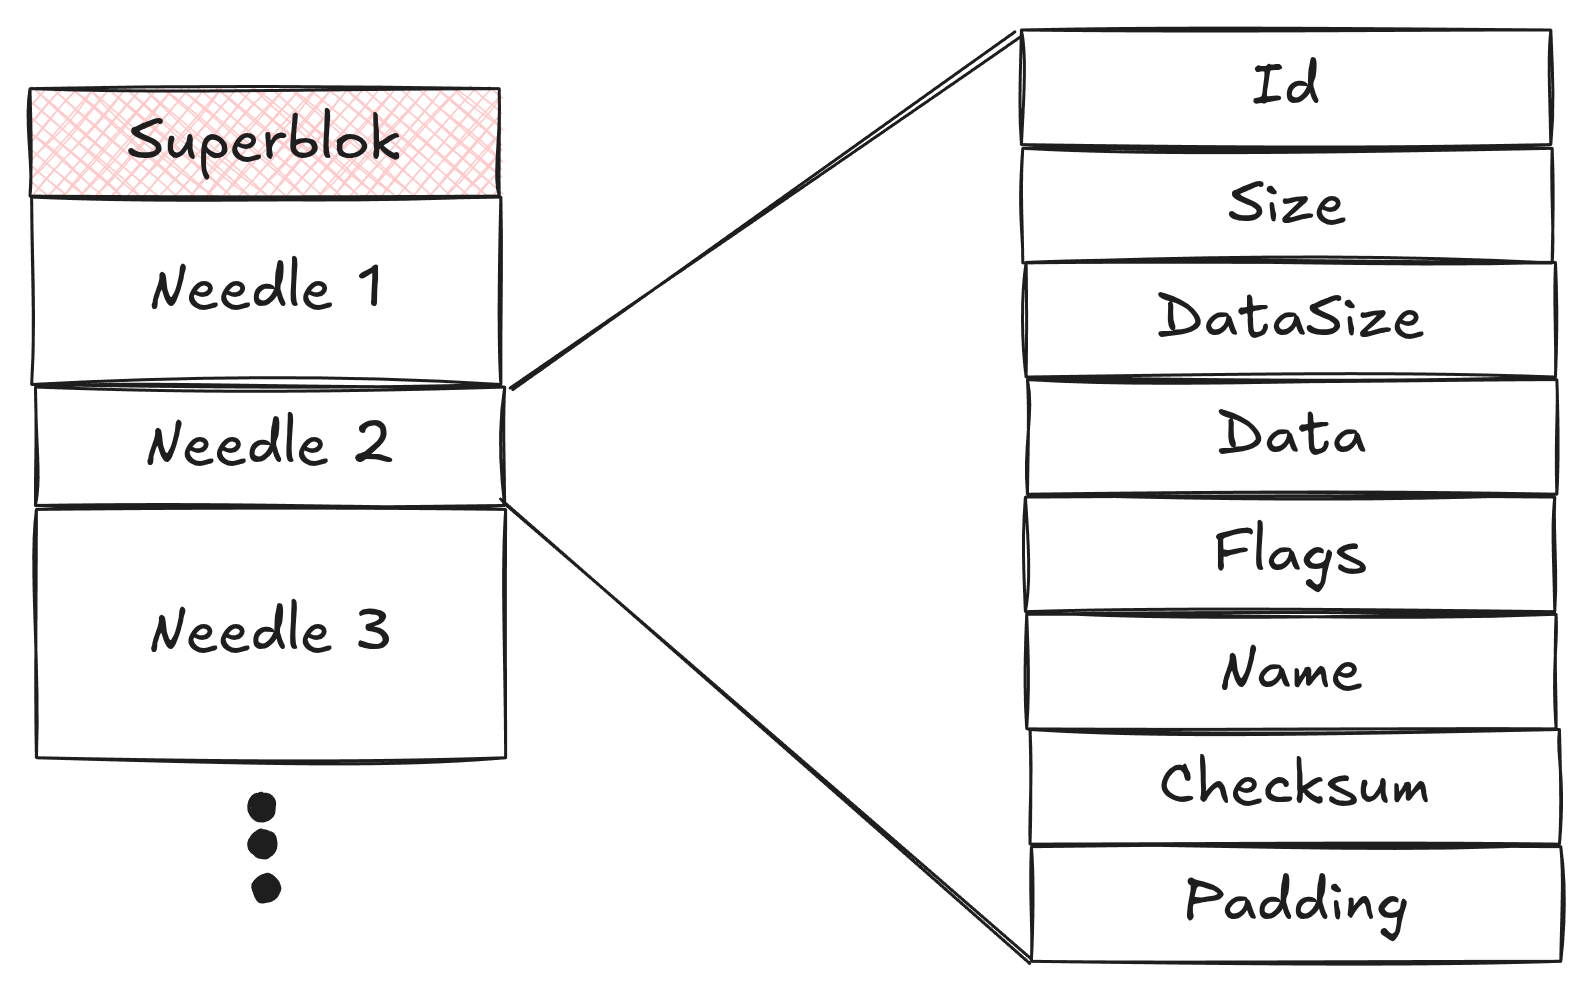
\includegraphics[width=0.6\textwidth]{images/seaweed-volume.png}
    \caption[SeaweedFS needle structure]{
      \label{fig:s-volume}
      SeaweedFS needle structure \\
      \cite{seaweedfs_authors_seaweedfsseaweedfs_2026}
      (\texttt{weed/storage/needle/needle.go)}
    }
\end{figure}

Such a volume-based architecture effectively transforms the problem of many small files into a few large ones. There are typically multiple of volumes on one system (node). \cite{beaver_finding_2010}

The organization of needles, reading, writing, and other operations are performed by a daemon running on the system. Such a system keeps opened file descriptors for each volume on the server and operates them as required. To effectively maintain volumes and needles on them, the service holds the so-called indexes. An index is a list of needles for each volume, each containing the offset and size of that needle, so they can be effectively addressed within volumes. Structure and architecture of the index can be seen in Figure \ref{fig:s-index}. When accessing the needle, the service presents an ID for the needle that encodes the needle's volume and ID.

\begin{figure}[h!t]
    \centering
    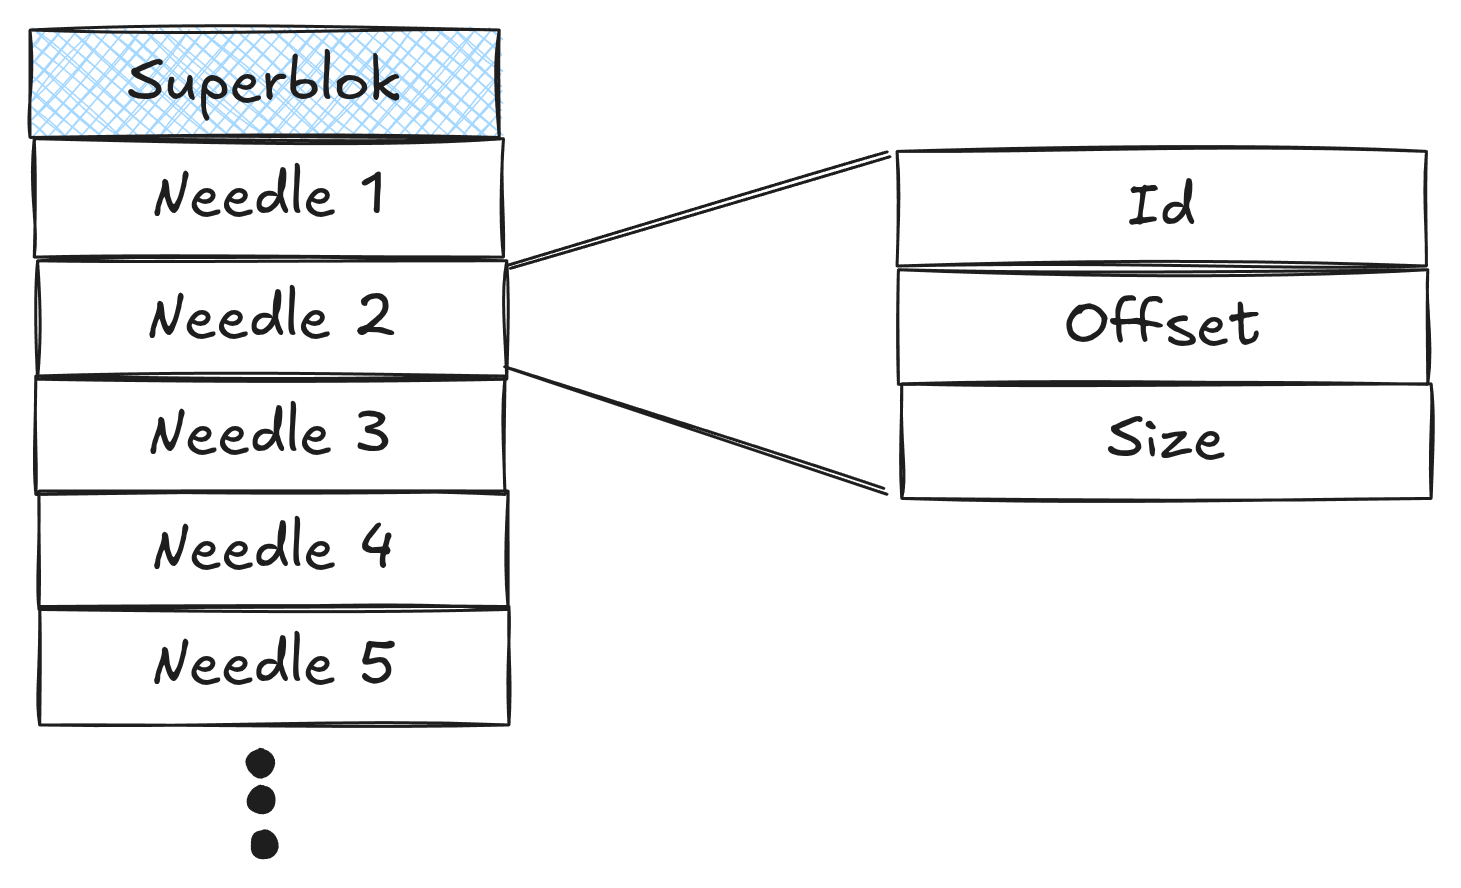
\includegraphics[width=0.6\textwidth]{images/seaweed-index.png}
    \caption[SeaweedFS needle index structure]{
        \label{fig:s-index}
        SeaweedFS needle index structure \\
        \cite{seaweedfs_authors_seaweedfsseaweedfs_2026}
        (\texttt{weed/storage/needle\_map/needle\_value.go})
    }
\end{figure}

Since an index is a collection of small data structures (in the SeaweedFS implementation, 16B), it is possible to keep all necessary data for addressing in the process's (data plane) main memory, thereby overcoming the problem of metadata overhead. It may seem that such a solution may be resource-intensive in the case of main memory. To manage 2,000,000 images, each 50 MiB in size (100 GiB in total), only $\approx$32 MB ($2*10^6 * 16B$) of main memory is required. 

Such a design of storing images as immutable objects in append-only mode introduces limitations, one of which is the inability to update or quickly delete a needle in storage. All limitations are not problematic in the context of image storage. Discussions for such limitations can be explored in detail in the Facebook Haystack paper. \cite{beaver_finding_2010}

\vspace{1.5em}

The design for managing metadata and files (needles) above is a common solution for the Haystack and SeaweedFS systems. It provides a detailed explanation of how the data plane of such systems works. In the SeaweedFS implementation service, the volume and metadata are referred to as weed volume. Another component called a master service is introduced. Since information about the implementation of the master server in the Haystack system is limited, from now on, only the SeaweedFS implementation will be discussed.

The master server is a component that orchestrates volume servers, creates volumes and enforces specified QoS. The master server operates on volumes as atomic units, treating them as if it did not know their structure. Replication, allocation, and other QoS are handled at the whole-volume level. In a replication setup, the master elects the master volume, which is the leader and append-enabled. This volume is used for appending. Read operations may be handled by multiple replicas based on the volume pool state. Any recovery and fault tolerance is also handled at volume levels. \cite{seaweedfs_seaweedfs_2024}

SeaweedFS implementation provides full access to Kubernetes, POSIX, S3, Hadoop, and WebDAV interfaces. For data durability, mainly replication is used, but erasure coding is also supported. Concrete abilities will be discussed in practical part of this thesis. \cite{seaweedfs_seaweedfs_2024}

\vspace{1.5em}
In summary, SeaweedFS addresses the specific scalability challenges associated with storing billions of small files. By adopting the Haystack architecture's approach of reducing disk I/O to Θ(1) and managing metadata in memory, it achieves high throughput with minimal overhead. It is an ideal choice for high-volume blob stores, content delivery networks, and data lakes where raw performance and storage efficiency are prioritized over the complex feature sets of general-purpose systems like Ceph.
